% V28 independently attested retrospective per-epoch identity technical companion, not new independent target validation.
% Original frozen cohorts and one newly executed but post-outcome Shin2017A comparator; see evidence hierarchy.
% Compile in paper_vnext, source files remain original and editable.
\documentclass[11pt,a4paper]{article}
\usepackage[margin=0.92in]{geometry}
\usepackage[T1]{fontenc}
\usepackage{amsmath,amssymb,booktabs,graphicx}
\usepackage{tikz}
\usepackage[hidelinks]{hyperref}
\usepackage{lmodern}
\usepackage[protrusion=true,expansion=false]{microtype}
\title{When Regularisation Selection and EEG Epoch Identity Matter:\\
Source Optimisation, Predictive Validation, and Transfer Discrepancy in EEG}
\author{AUTHOR IDENTITIES AND AFFILIATIONS TO BE APPROVED}
\date{}
\begin{document}
\maketitle
\begin{abstract}
\textbf{Objective:} Covariance-fitting fidelity,
predictive likelihood and source-participant
discrimination are distinct objectives for
EEG regularisation. We test when their
selection disagreement changes unknown-person
decoding, and whether a more exact source
search resolves the discrepancy.
\textbf{Methods:} We retain a source-fitted
covariance/tangent-LDA pipeline, participant-grouped
selection and source-only target information
boundaries. We correct a validation class-centred
covariance score to genuine source-trained-mean
Gaussian predictive likelihood, and decompose
AUC changes into positive--negative pair transitions.
Spectral interval bounds are used to search
continuous shrinkage ranges while reporting
conditional source-only optimality gaps.
\textbf{Results:} In a frozen EEGMMIDB
20-person block, source-discrimination selection
exceeded the historical class-centred score
by $0.0561$ AUC (Holm $p=0.00597$), although
five participants were harmed by more than
0.02 AUC. A three-channel BNCI2014\_004
worst-quarter source-risk criterion changed
eight of nine selections without a mean
AUC improvement. An anchored BNCI2014\_002
source search reduced an inconclusive
continuous-source optimality gap from
0.09477 to 0.01623 without improving
the original grid AUC. In a separate
protocol-first, unregistered Weibo2014
test (ten participants, 1,580 trials),
the continuous selector met its source
tolerance in all ten pools yet selected
the same shrinkage as the 27-point grid
in every pool; both obtained
0.73141 held-person macro AUC.
The gain relative to proper Gaussian
selection was only $0.00205$ AUC.
\textbf{Conclusion:} Closing a source
optimisation gap need not reduce transfer
risk. Correct validation estimands,
selection chronology and participant-level
negative results matter more than
shrinkage-grid precision alone.
\end{abstract}

\noindent\textbf{Keywords:} EEG; covariance shrinkage; cross-subject decoding;
motor imagery; model-selection validity; representation sensitivity.

\section{Introduction}
Cross-subject EEG decoding asks a model fitted on source participants to
generalise to a different individual, often without labelled calibration.
Tangent-space covariance features are established in EEG decoding
\cite{barachant2012riemannian}, and can be high dimensional even
when each participant contributes few examples. A stable covariance estimator is therefore
attractive, but the statistical criterion used to estimate a covariance
matrix is not the criterion used to judge held-person classification.
Ledoit--Wolf shrinkage is an established covariance estimator
\cite{ledoit2004}; regularised discriminant analysis selected against
predictive discrimination is also classical \cite{friedman1989}.
Consequently, selecting a shrinkage parameter by source discrimination
is not, in itself, our claimed methodological invention.

A more basic measurement question is what is actually being scored:
centring held source participants with their own class means produces a
covariance log score that does not equal the predictive Gaussian log score
under source-trained means. Confusing these objectives can create an
apparent advantage for discrimination-based selection. A corrected
comparator must be run on real EEG to determine whether the original
objective comparison survives. A separate prospective intervention asks
whether the selection criterion can alter a spectral representation
conclusion under the same target-information budget. Contemporary work proposes
new regularisation mechanisms and multi-paradigm transfer methods
\cite{miao2025freezing,morvay2026wbt,he2026cyclic}, while recent research highlights
how participant-level rather than trial-level evaluation can change the
interpretation of EEG model performance \cite{gil2026subjectvalidation}.
Qin and colleagues, in a recent study published in this journal,
evaluated spatial normalization with SVM decoding across nine
distinct EEG paradigms under within- and between-subject validation
\cite{qin2026spatialnorm}. That study provides stronger
cross-paradigm breadth than the fixed tangent-LDA family examined here.
Our narrower, complementary question is how the \emph{source
validation likelihood itself} changes the selected
regularisation regime; this is a measurement problem rather
than evidence of a superior novel classifier.
These contributions motivate our strict comparison but do not substitute
for an objective-controlled study.

We study a fixed tangent-space linear discriminant family, separating
three source-only selection targets: held-source-participant
macro-AUC, a validation-class-centred covariance score, and a true
Gaussian predictive score using only source-training class means.
The third comparator was executed on Shin2017A only after its original
target results had been seen; this is retrospective and is not part of
the frozen confirmatory family. All target labels, target feature
moments and target-fitted geometry are excluded from primary source-only
(Z0) selection. We preserve the original predeclared finite shrinkage grid,
frozen prospective test cohorts, the representation falsification,
individual harms, and the newly verified posterior comparator. An additional BNCI2014\_001 acquisition and a new Weibo2014
ten-person, three-channel dataset were evaluated under
repository-committed protocol-first procedures. Neither experiment
constitutes independent external preregistration.

The objective is not to show
that one numerical shrinkage value is universally optimal; it is to measure
how an incorrectly described covariance-validation estimand can change
the interpretation of a transfer comparison.


\subsection{Relation to current cross-subject EEG validation research}
This study complements, rather than replaces, the development of
spectral filters, classifiers and adaptation methods. Recent
cross-subject EEG work has demonstrated that window- or trial-level
performance estimates can differ considerably from genuine
unseen-participant performance \cite{gil2026subjectvalidation}. A
separate 45-person mental-workload study has shown that feature
representation, model class and the allowance for subject-specific
calibration can also strongly affect generalisation
\cite{abinaya2026wavelet}. Both results caution against evaluating
one model under a more favourable target-information budget than
another. They do not directly answer the within-pipeline question
of whether selecting \emph{the same} scalar regulariser by
covariance predictive likelihood or by source-person
discrimination changes which EEG representation appears better.

We deliberately keep the comparison narrower than studies introducing
new classifiers. The use of target-person unlabeled moments,
target-conditional geometry, entropy minimisation or a few labeled
calibration trials may benefit model adaptation, but changes the
information contract. A Z0 result cannot be directly ranked against
one of these adapted classifiers as if the procedures used the same
information. In this article, Ledoit--Wolf, OAS and source
covariance-NLL are estimator/objective controls; Riemannian MDM,
tangent logistic regression and a separate CSP6 classifier
are architectural reference points. Comparing those latter
representations does not prove a new state-of-the-art BCI decoder.

The essential methodological contrast is between \emph{estimation
quality of a covariance operator} and \emph{out-of-person
discrimination of a derived decision direction}. The mathematical
non-equivalence is familiar from regularised discriminant analysis
\cite{friedman1989}; our empirical contribution is its prospective,
participant-level consequence, including a spectral representation
hypothesis that the new results contradict. This framing prevents
a conventional parameter-selection strategy from being presented
as a newly invented learning algorithm.


\section{Methods}
\subsection{Datasets and target-information budgets}
PhysioNet EEGMMIDB S001--S008 is the method-development source pool
\cite{schalk2009eegmmidb,schalk2004bci2000}.
Its S021--S040 participants form a prospectively untouched target block
of 20 people. The primary fixed 21-channel sensorimotor montage, 8--30 Hz
filtering and source-fitted Riemannian tangent reference generate 231
wide-band coordinates. The independently frozen BNCI2014\_002
(\(N=14\), 15 channels, 120 features) and BNCI2015\_001
(\(N=12\), 13 channels, 91 features) protocols use native montage,
8--30 Hz processing and leave-one-person-out evaluation. Shin2017A
(\(N=29\), 30 channels, 465 features) was frozen under a \emph{separate}
prospective protocol before that cohort's target outcomes and is not a
retrospective addition to the original BNCI inference family.

All main effects use Z0: no target labels, target feature means, target
covariance, target normalisation statistics or target-selected feature
configuration. Within each source-validation fold, tangent references and
other representation-dependent operations are refitted using available
source participants only. Repeated trials and sessions do not become
independent inferential units.

\subsection{Paired objectives on one scalar shrinkage path}
For source within-class covariance \(S\), let
\[
 A_\lambda=(1-\lambda)S+\lambda\nu I,\qquad
 \nu=\mathrm{tr}(S)/p,\quad \lambda\in[0,1].
\]
Two source objectives are evaluated on the same participant-grouped folds:
macro-AUC \(A_s(\lambda)\), maximised for discrimination, and held-source validation-class-centred covariance log score
\(C_s(\lambda)\), minimised for within-class covariance fit.
This frozen estimator historically appears in logs and tables as
Cov-NLL, but it uses each held-source validation participant's own
class-centred residuals; it is not a source-mean predictive likelihood
(Section~\ref{sec:v16-estimand-audit}). Analytic Ledoit--Wolf and OAS shrinkage use the same
source feature pool; tangent-space logistic regression and Riemannian
MDM serve as additional non-identical algorithm controls. Full-domain
selection refers to the \emph{finite} 27-point candidate grid
\[
\begin{aligned}
\Lambda=\{&0,.0005,.001,.002,.003,.005,.0075,.01,.015,\\
&.02,.03,.05,.075,.10,.15,.20,.30,.40,.50,\\
&.60,.70,.80,.90,.95,.98,.99,1\}.
\end{aligned}
\]
Singular candidates are declared infeasible, not silently replaced by
a target-informed rule. Target scores are frozen before their
label-based performance is calculated.

\subsection{A critical estimand distinction: class-centred covariance score versus predictive NLL}
\label{sec:v16-estimand-audit}

An audit of the \emph{original executed} Shin2017A/BNCI2014\_002
source-selection code found a material distinction between the
frozen baseline's historical name and its actual measurement
quantity. The original program performs source-participant-grouped
validation, forms within-class residuals from \emph{the held source
validation participant's own labelled class means}, and evaluates
a covariance Gaussian log score on those residuals.
These source-participant labels are permitted for model development
and do \emph{not} imply outer target-subject label leakage.
However, the resulting number is not a proper predictive
class-conditional log likelihood under source-fitted class means.

To be precise, write the source-trained regularised within-class
covariance as $A_\lambda$, and for held source participant $g$
let $\widehat\mu_{g,c}$ be the \emph{held} participant's
empirical mean for class $c$. Up to additive constants, the
original finite-sample validation score is
\begin{equation}
\label{eq:v16-centred-score}
 C_{\mathrm{cent},g}(\lambda)=\frac{1}{p}
 \left[
  \log|A_\lambda|+
  \frac{1}{n_g}\sum_{i=1}^{n_g}
  (x_{gi}-\widehat\mu_{g,y_{gi}})^\top
  A_\lambda^{-1}(x_{gi}-\widehat\mu_{g,y_{gi}})
 \right].
\end{equation}
The source criterion in the frozen experiments is the
grouped average of $C_{\mathrm{cent},g}(\lambda)$,
and all existing performance tables retain its original
method identifier \texttt{source\_cov\_nll\_full\_domain\_LDA}.
For readability we call it the
\emph{class-centred covariance-score selector (CovScore)}
hereafter. Historical Cov-NLL column labels refer
to this exact frozen estimator, not to the new comparator below.

A \emph{genuinely held-source predictive} Gaussian
class-conditional score would instead evaluate
\begin{equation}
\label{eq:v16-conditional-prediction}
 C_{\mathrm{pred},g}(\lambda)=\frac{1}{p}
 \left[
  \log|A_\lambda|+
  \frac{1}{n_g}\sum_{i=1}^{n_g}
  (x_{gi}-\widehat\mu_{\mathrm{train},y_{gi}})^\top
  A_\lambda^{-1}(x_{gi}-\widehat\mu_{\mathrm{train},y_{gi}})
 \right],
\end{equation}
with the class means and covariance fitted from
\emph{the source training groups only}, without refitting
the held group's means. The source-validation labels
index the corresponding training-class mean; they are
not used to estimate it. Equation~\eqref{eq:v16-conditional-prediction}
is a different comparison protocol, \emph{not}
the estimand evaluated in the original frozen
EEGMMIDB/BNCI/Shin result tables. A later \emph{post-outcome}
real EEG execution of this corrected source-only criterion
on Shin2017A is reported separately in
Section~\ref{sec:v18-fair-predictive}; it is not
part of any original prospective testing family.

\paragraph{Proposition (class-contrast shift blind spot).}
Consider any fixed held-source validation data with
at least one observation in each class, and apply an
arbitrary class-specific feature translation
$x'_{gi}=x_{gi}+b_{y_{gi}}$.
Then \emph{for every feasible} $\lambda$,
\[
 C'_{\mathrm{cent},g}(\lambda)
 = C_{\mathrm{cent},g}(\lambda).
\]
In contrast, $C_{\mathrm{pred},g}$ is generally changed
because the source-trained class means stay fixed.
Consequently, $C_{\mathrm{cent}}$ by construction
cannot measure conditional mean-contrast drift through
its held-source covariance log score.

\emph{Proof.} After translation,
$\widehat\mu'_{g,c}=\widehat\mu_{g,c}+b_c$,
so each residual
$x'_{gi}-\widehat\mu'_{g,y_{gi}}=
x_{gi}-\widehat\mu_{g,y_{gi}}$
is identical to its original value. The log-determinant
term does not depend on the held means. For the
predictive score, the source-fitted
$\widehat\mu_{\mathrm{train},c}$ does not shift and
the residual gains $b_c$ in general, changing its
quadratic form.\hfill$\square$

An exact numerical regression now computes both quantities
on identical synthetic training/validation splits, then
imposes class-conditional shifts. The historical
class-centred score remains equal to floating-point
precision along the entire $\lambda$ path, while
proper predictive log score changes. This
\emph{does not} prove that one of the two selectors
will improve EEG transfer; such a claim would require
a fresh source-only, pre-specified, held-person
experiment with the new comparator.

\paragraph{Interpretational consequence.}
The prospective finding in the present paper remains
a comparison of \emph{source participant discrimination}
against \emph{class-centred covariance fit} and
against analytic Ledoit--Wolf. The measured gain
relative to the frozen Cov-NLL code remains
numerically unchanged, but should no longer be described
as showing superiority over every possible covariance
predictive likelihood criterion.
This distinction also restricts the operator mechanism:
the derivative of the covariance quadratic form
is a conditional calculation at a fixed covariance,
not evidence that Eq.~\eqref{eq:v16-centred-score}
evaluates out-of-sample class-conditional density
with source-only class means. Source-only diagnostics
from the two definitions must never share an
ambiguous NLL field without their
residual-centring provenance.


\subsection{The exact missing term in the historical covariance-score criterion}
\label{sec:v17-mean-shift-decomposition}
The distinction between a validation-class-centred Gaussian
covariance score and a genuine source-trained-mean predictive
log score can be made \emph{exact}, rather than relying only
on a synthetic translation counterexample.

For one held \emph{source} validation person $g$ with $n_g$
examples in $p$ dimensions, let
$\widehat\mu_{g,c}$ denote its empirical class means,
$\widehat\mu_{\mathrm{train},c}$ the means fitted exclusively
on the source-training people, and
$\Delta_{g,c}=\widehat\mu_{g,c}-
\widehat\mu_{\mathrm{train},c}$. For any common,
source-fitted positive definite regularised covariance
$A_\lambda$, the two V16 criteria satisfy
\begin{equation}
\boxed{
 C_{\mathrm{pred},g}(\lambda)
 =
 C_{\mathrm{cent},g}(\lambda)
 +\frac{1}{p}\sum_{c\in\{0,1\}}
 \frac{n_{g,c}}{n_g}
 \Delta_{g,c}^\top A_\lambda^{-1}\Delta_{g,c}.
}
\label{eq:v17-exact-nll-shift}
\end{equation}
The additional term is \emph{nonnegative} and
becomes zero exactly when the validation class means
match the training class means, for all classes present.
It is a covariance-weighted \emph{source-person
class-mean shift penalty}, not a regularisation
term chosen by target data.

\emph{Proof.} For each validation trial of class $c$,
decompose
$x_{gi}-\widehat\mu_{\mathrm{train},c}=
(x_{gi}-\widehat\mu_{g,c})+\Delta_{g,c}$.
Expand the quadratic form under $A_\lambda^{-1}$.
The cross term vanishes within each class because
$\sum_{i:y_i=c}(x_{gi}-\widehat\mu_{g,c})=0$.
Both log-determinant terms agree, and the remaining
class-mean quadratic terms give
Eq.~\eqref{eq:v17-exact-nll-shift}.\hfill$\square$

The penalty is $\lambda$-dependent because it measures
class-mean drift in the metric induced by $A_\lambda^{-1}$.
Its derivative can have \emph{either} sign:
\[
 \frac{\partial}{\partial\lambda}
 \bigl(C_{\mathrm{pred},g}-C_{\mathrm{cent},g}\bigr)
 =-\frac1p\sum_c\frac{n_{g,c}}{n_g}
 \Delta_{g,c}^\top A_\lambda^{-1}
 (\nu I-S)A_\lambda^{-1}\Delta_{g,c}.
\]
It follows that the proper predictive criterion
can select more \emph{or} less shrinkage than
the class-centred comparator. Merely asserting
that predictive selection is stronger or always
more regularised is unsupported. An independent
executable test verifies the identity for 300
randomly generated full-rank covariance operators,
multiple feature dimensions and source/validation
class-mean shifts, without using any held outer
target EEG data.

The identity provides a mechanistic interpretation
of the V16 estimand audit: the old frozen covariance
selection scores how well $A_\lambda$ describes
\emph{within-class residual fluctuations} in a
held source person; the correctly predictive version
also penalises \emph{between-source-person class-mean
misalignment}. This is not a newly invented
covariance estimator, and it does not establish that
minimising the added penalty improves held-person AUC.
A real, correctly nested evaluation of this second
source-selection criterion remains essential.


\subsection{Operator explanation and safe diagnostics}
Writing source class contrast \(d_s\), the discriminant is
\(w_\lambda=A_\lambda^{-1}d_s\) and
\[
 w_\lambda'=-A_\lambda^{-1}(\nu I-S)w_\lambda.
\]
For held-participant covariance \(\Sigma_g\) and class contrast \(d_g\),
consider standardized signed margin
\(m_g=w_\lambda^\top d_g/\sqrt{w_\lambda^\top\Sigma_gw_\lambda}\).
Subtract the component of \(w_\lambda'\) that merely rescales the
discriminant in the \(\Sigma_g\) metric, defining
\[
 r_g=w_\lambda'-
 \frac{w_\lambda'^\top\Sigma_gw_\lambda}
 {w_\lambda^\top\Sigma_gw_\lambda}w_\lambda.
\]
Differentiation yields
\[
 m_g'(\lambda)=
 \frac{r_g^\top d_g}{\sqrt{w_\lambda^\top\Sigma_gw_\lambda}}.
\]
The covariance quadratic-form derivative contains covariance operators but
not class contrast, conditional on a fixed covariance; the empirical
validation-class-centred score must not be called predictive likelihood. Thus a stationary covariance-fidelity optimum need not
be stationary for the held-person margin. Around an \emph{interior} covariance
optimum, covariance regret can be second-order while margin change is
first-order; this local statement is not assumed at boundary optima.

To describe objective disagreement without constructing an unstable ratio,
we preserve both source-only regret paths:
\[
 R_C(\lambda)=C_s(\lambda)-\min_\ell C_s(\ell),\quad
 R_D(\lambda)=\max_\ell A_s(\ell)-A_s(\lambda).
\]
Their cross-optimum values, together with source-only covariance-metric
discriminant rotation, quantify a descriptive conflict.
These are \emph{not} validated target-gain predictors. A new auditable
implementation is provided separately with synthetic unit tests; no
target outcomes are used to set its threshold.

\subsection{AUC-active regularisation changes: an exact rank-transition audit}
\label{sec:v22-rank-transitions}
A difference between two selected shrinkage parameters does not itself
measure a downstream prediction difference. Nor does rotation of the
discriminant vector necessarily modify the ranking of positive and negative
trials. We therefore distinguish a \emph{selection change}, a
\emph{score-order change}, and a \emph{signed AUC change}. This section
provides a transparent diagnostic identity and a falsifiable source-only
analysis protocol; it does not introduce a previously validated novel
classifier or an independently confirmed predictive certificate.

For participant $g$ with positive trials $P_g$ and negative trials $N_g$,
let $z_{pn}(\lambda)=f_\lambda(x_p)-f_\lambda(x_n)$ and
$h(z)={\bf1}\{z>0\}+\tfrac12{\bf1}\{z=0\}$. Then
\[
  A_g(\lambda)=\frac{1}{|P_g||N_g|}
     \sum_{p\in P_g,n\in N_g}h(z_{pn}(\lambda)).
\]
For source-only decisions $a,b$, count pair-state transitions in a
$3\times3$ matrix $M_{ij}^{(g)}(a,b)$ where
$i,j\in\{-,0,+\}$ describe the signs of $z_{pn}(a),z_{pn}(b)$.
With credit vector $c=(0,\tfrac12,1)$, the following identity is exact,
including score ties:
\begin{equation}
  A_g(b)-A_g(a)=
  \frac{\sum_{i,j}M_{ij}^{(g)}(a,b)(c_j-c_i)}
       {|P_g||N_g|}.
  \label{eq:v22-exact-pair-transition}
\end{equation}
Gross pair-state churn
$G_g(a,b)=\sum_{i\ne j}M_{ij}^{(g)}(a,b)/(|P_g||N_g|)$
may be nonzero or large although the \emph{signed} difference in
Eq.~\eqref{eq:v22-exact-pair-transition} is zero. Thus parameter
disagreement and even extensive pairwise reordering are insufficient to
claim improved discrimination. This basic rank identity is not claimed
as a new mathematical theorem. Its value here is an exact, inspectable
link between the original covariance--discrimination mismatch and the
observed possibility of near-invariant ROC-AUC.

For source validation, matrices and AUCs are computed for each
held-\emph{source} participant using only an inner model trained on
different source participants. We report participant-macro averages of
$G_g$ and the signed differences, rather than pooling pairs across
participants of unequal trial counts. The original source-only choices
are computed first, and no outer target record enters the source
diagnostic. Any application of Eq.~\eqref{eq:v22-exact-pair-transition}
to frozen outer target scores is a \emph{post-outcome explanation}, not
an admissible selection or early-warning rule. In particular, exactness
of the decomposition does not give a finite-sample confidence bound for
future participants or justify treating overlapping source folds as
independent.

\paragraph{Mechanistic promotion test.}
The frozen V21 BNCI2014\_004 observation---eight of nine CVaR selections
different from source macro selection without a mean AUC or
material-harm improvement---motivates the diagnostic, but does not
validate it. Source pair-churn, cancellation, and subject dispersion
must be compared against scalar $\lambda$ distance, source AUC regret,
covariance regret, and source discriminant rotation on a separately
untouched external acquisition before making a predictive or improved
target-AUC claim. We retain all false alarms, missed harms, and negative
results. An executable implementation, leakage-contract tests, and the
pre-outcome falsification protocol accompany the research draft.

\subsection{A conditional spectral enclosure of AUC change over a continuous shrinkage path}
\label{sec:v23-spectral-continuum}
The finite endpoint transition decomposition in
Section~\ref{sec:v22-rank-transitions} can identify rank changes
\emph{after} two scalar-shrinkage choices have been evaluated.
A more demanding question is whether a ranking remains unchanged for
\emph{every} regularisation value on the interval between them.
We exploit the existing source-trained LDA eigensystem, not a
new classifier. For fixed source-trained class contrast $d_s$,
$S=U\operatorname{diag}(s_i)U^\top$ and
$A_\lambda=(1-\lambda)S+\lambda\nu I$,
the score difference on a positive--negative pair of held
\emph{source-validation} trials with vector difference $v_{pn}$ is
\begin{equation}
 z_{pn}(\lambda)=v_{pn}^\top A_\lambda^{-1}d_s
 =\sum_{i=1}^p\frac{(u_i^\top v_{pn})(u_i^\top d_s)}
 {(1-\lambda)s_i+\lambda\nu}.
 \label{eq:v23-spectral-path}
\end{equation}
Every candidate is required to have a positive denominator over the
entire interval. For any subinterval $[l,r]$ and coefficient
$a_{i,pn}=(u_i^\top v_{pn})(u_i^\top d_s)$, each individual rational
summand is monotone because its denominator is affine and strictly
positive. Hence for all $\lambda\in[l,r]$,
\begin{align}
 L_{pn}[l,r]&=\sum_i\min\left\{
 \frac{a_{i,pn}}{(1-l)s_i+l\nu},
 \frac{a_{i,pn}}{(1-r)s_i+r\nu}\right\},\nonumber\\
 U_{pn}[l,r]&=\sum_i\max\left\{
 \frac{a_{i,pn}}{(1-l)s_i+l\nu},
 \frac{a_{i,pn}}{(1-r)s_i+r\nu}\right\},
 \label{eq:v23-interval}
\end{align}
enclose $z_{pn}(\lambda)$ as
$L_{pn}[l,r]\le z_{pn}(\lambda)\le U_{pn}[l,r]$.
Consequently, if every subinterval has $L_{pn}>0$, that pair
remains positive throughout the complete path; similarly if
every subinterval has $U_{pn}<0$, its sign remains negative.
Pairs that fail the test are \emph{uncertain}, not observed
reversals. We additionally intersect the termwise enclosure
with a centered second-order Taylor interval.
For $m=(l+r)/2$, $h=(r-l)/2$, define
$z_m=z_{pn}(m)$, $z'_m$ from the spectral derivative,
and the curvature envelope
\[
 B_{2,pn}[l,r]=
 2\sum_i\frac{|a_{i,pn}|(\nu-s_i)^2}
 {\min\{(1-l)s_i+l\nu,(1-r)s_i+r\nu\}^{3}}.
\]
Taylor's theorem implies
\[
 z_{pn}(\lambda)\in
 [z_m-R_{pn},z_m+R_{pn}],\quad
 R_{pn}=h|z'_m|+\tfrac12h^2B_{2,pn}[l,r].
\]
Intersecting the two valid intervals retains the enclosure
while exploiting first-derivative cancellation. This refinement
was developed \emph{after} the first continuous-search pilot
showed a loose residual gap and is not an independently
prospectively confirmed improvement.

\paragraph{Finite-trial AUC sensitivity bound.}
For a fixed validation person $g$, denote by $\eta_g$
the fraction of positive--negative trial pairs not certified
strictly sign-stable over the whole interval. Since every
certified pair contributes unchanged AUC credit $0$ or $1$
throughout, while each uncertified pair may vary by no more
than one unit of credit, for all $\lambda\in[l,r]$,
\begin{equation}
 \left|A_g(\lambda)-A_g(l)\right|\le\eta_g.
 \label{eq:v23-continuum-bound}
\end{equation}
This is a deterministic bound on a fixed participant's fixed
sample scores, conditional on the computed source eigensystem;
it is \textbf{not} an unseen-person generalisation guarantee
or a statistical confidence interval. The mathematical
ingredients---spectral shrinkage and scalar interval arithmetic---
are standard. We do not claim novelty for either ingredient.
In implementation, a conservative floating-point
slack prevents a near-zero pair from receiving a fragile
rank-stability certificate; without machine-verified directed
rounding we do not claim formal verified-numerics correctness
for the original real-valued dataset.

The procedure is evaluated on source-validation subjects
under the same original fixed EEG covariance and
tangent-space folds as V21--V22. The candidate $\lambda$
endpoints are computed from SOURCE people only; no outer
target data enter this analysis. Crucially, decreasing
the bound in Eq.~\eqref{eq:v23-continuum-bound}
is a property of the source trial-score path, not evidence
that a future target subject will be protected. To promote
this analysis to a novel useful model-selection policy
requires a frozen source-statistic-to-selection map and an
unexposed external acquisition that tests actual target harm.

\subsection{Continuous source-only regularisation search with an auditable optimisation gap}
\label{sec:v23-continuous-search}
The source rank enclosure in Eq.~\eqref{eq:v23-interval} also
makes it possible to search a \emph{continuous} shrinkage interval,
instead of interpreting success on a finite grid as
optimality across $\lambda\in[0,1]$.
This is a computational claim about the \emph{fixed,
held-source-validation} macro-AUC, not a generalisation bound
for unseen participants.

For each grouped source fold, fix the source-fitted
covariance eigensystem, contrast and held-source feature/label
pairs. On subinterval $I=[l,r]$, identify the uncertified
positive--negative pairs with indicator $J_{pn}(I)$.
Let $c_{pn}(l)\in\{0,\tfrac12,1\}$ be their AUC credit
at the left endpoint. For every $\lambda\in I$,
\begin{equation}
 A_g(\lambda)\le A_g(l)+
 \frac{\sum_{pn}J_{pn}(I)[1-c_{pn}(l)]}{|P_g||N_g|}.
 \label{eq:v23-one-sided-auc-upper}
\end{equation}
The corresponding lower bound subtracts
$\sum_{pn}J_{pn}(I)c_{pn}(l)/(|P_g||N_g|)$.
Averaging bounds \emph{per source person} encloses
the macro-AUC objective across the full interval,
including nonsampled shrinkage parameters.

A reproducible branch-and-bound search bisects
the interval with largest remaining source-macro upper
bound, evaluates AUC at a midpoint, and updates the
incumbent. It stops with an $\epsilon$-source
optimality certificate only if the best unresolved
interval bound exceeds the best evaluated source AUC
by at most $\epsilon$. Exhausting an evaluation
budget earlier yields an \emph{inconclusive} result,
with its unclosed gap reported.
No held target label enters any selection or stopping rule.

Classical interval arithmetic, branch-and-bound and LDA
shrinkage are prior art. The domain-specific methodological
extension is an inspectable finite-\emph{source}-AUC
optimality gap across a continuous shrinkage range,
rather than an automatically superior EEG classifier.
The scientific question of future-person generalisation
remains open until a frozen external EEG test.

\subsection{Separating source optimisation error from transfer error}
\label{sec:v24-selection-gap}
The V23 continuous-path enclosure constrains the maximum
\emph{source-validation} macro-AUC; it does not constrain the
performance of an unseen target participant. This distinction can
be made precise using a simple deterministic inequality.

Let $S(\lambda)$ be the participant-macro AUC of frozen
held-source validation scores, and $T(\lambda)$ the AUC on
a fixed unseen target participant, on a common feasible candidate
set $\Lambda$. Suppose a source-only selector chooses
$\widehat\lambda$ with
\[
 \max_{\lambda\in\Lambda} S(\lambda)
   -S(\widehat\lambda)\le\varepsilon_S.
\]
Define the unobservable-at-selection transfer discrepancy
\[
 \Delta_{S,T}(\Lambda)=
 \sup_{\lambda\in\Lambda}|S(\lambda)-T(\lambda)|.
\]
Then a direct add-and-subtract argument gives
\begin{equation}
 \underbrace{\max_{\lambda\in\Lambda}T(\lambda)
   -T(\widehat\lambda)}_{\text{target-oracle regret}}
 \le \underbrace{\varepsilon_S}_{\text{source selection gap}}
 +\underbrace{2\Delta_{S,T}(\Lambda)}_{\text{source--target discrepancy}}.
 \label{eq:v24-transfer-gap}
\end{equation}
This elementary inequality is not a newly discovered statistical
generalisation theorem. Its contribution to the study is to make
explicit \emph{why better source optimisation alone may be
irrelevant to transfer}: closing the source optimisation gap does
not control the second term. A source-only certificate for
$\varepsilon_S$ therefore must not be reported as a guarantee
on Eq.~\eqref{eq:v24-transfer-gap}; target labels would be required
to compute $\Delta_{S,T}$ post hoc. Non-exchangeable and label-reversed
target populations can have the same observed source data but
conflicting best shrinkage decisions. No source-only selector can
promise universally improved target AUC without additional
assumptions.

\paragraph{Matched source search repair.}
The original V23 exploratory continuous optimiser started with two
interval endpoints and five bisections and therefore sometimes
failed to evaluate the original 27-point grid's best candidate
within the same interval. The V24 repair first evaluates the
\emph{predeclared source-only} feasible finite-grid candidates,
partitions the continuous interval at them and searches
subintervals with pair-credit upper bounds. This eliminates
a logically avoidable finite-grid regression, at the cost of
additional candidate evaluation; that cost is reported.

In a genuine BNCI2014\_002 held-source experiment (first
outer pool, 13 validation source people), the original grid
and the repaired continuous search both attained source
macro-AUC $0.79397$ with selected $\lambda=0.8$.
The computed conditional source upper bound decreased to
$0.81019$, so the remaining source-only optimum gap
was at most $0.01623$ within the fixed interval
$[0.05,0.95]$ under the numerical enclosure assumptions.
This met the predeclared 0.02 \emph{source} AUC tolerance,
but yielded \emph{zero observed source AUC improvement}
relative to the already competitive grid. The earlier
endpoints-only five-split search had source AUC $0.79296$
and an inconclusive $0.09477$ source optimality gap.
This is a repaired optimisation audit, not a new target
transfer gain or clinical safety certificate.

\paragraph{External decision gate.}
A new public MI acquisition (Weibo2014, 10 participants,
three fixed sensorimotor electrodes and binary left/right
imagery) is reserved by a repository-committed, pre-outcome
source-only first-run protocol. Four source-only comparators
and a fifth fixed-grid control are chosen before target
scores are evaluated. Successful execution and actual
participant-level target outcomes are required before any
algorithm-performance statement can appear in this
manuscript; an in-repository freeze is not equivalent
to an independent registry preregistration. If the anchored
search matches the 27-point baseline without target benefit,
we will retain the negative result rather than claim the
continuous optimiser is a superior transfer algorithm.

\subsection{Finite rank cells on the continuous spectral shrinkage path}
\label{sec:v25-bernstein-rank-cells}
The V23 interval method bounded source-trial score signs by
enclosing the individual rational terms. In low-dimensional
EEG, a complementary approach acts on their \emph{common
numerator}, exploiting cancellations otherwise lost in
termwise bounds.

For fixed source-trained eigensystem
$S=U\,\mathrm{diag}(s_1,\ldots,s_p)U^\top$, class contrast
$d_s$, fixed held-\emph{source} positive--negative feature
difference $v_{pn}$, let
\[
q_i(\lambda)=(1-\lambda)s_i+\lambda\nu,\qquad
a_{i,pn}=(u_i^\top v_{pn})(u_i^\top d_s).
\]
On a feasible interval $I$ where $q_i(\lambda)>0$ for all
$i,\lambda$, the sign of the score difference is the sign
of the single polynomial
\begin{equation}
 N_{pn}(\lambda)
 =\sum_{i=1}^{p}a_{i,pn}\prod_{j\ne i}q_j(\lambda),
 \qquad\deg N_{pn}\le p-1 .
 \label{eq:v25-spectral-numerator}
\end{equation}
Indeed $z_{pn}=N_{pn}/\prod_iq_i$ and the denominator is
strictly positive. Unless $N_{pn}$ vanishes identically
(and the pair remains tied throughout), a positive--negative
pair can change its strict ordering only at the at most
$p-1$ distinct real roots of $N_{pn}$. Hence the finite
source-validation macro-AUC is piecewise constant on
the complement of the finite union of all such rank-cell
boundaries. Values \emph{at} a root are evaluated separately
because ties count for one-half AUC credit; it would be
incorrect to assume the supremum is attained only at
open-cell midpoints. The root-count argument is an
elementary consequence of rational functions, not a
claim of priority for new polynomial algebra.

For each subinterval $[\ell,r]$, map $\lambda$ to
$t\in[0,1]$ and express the degree-$p-1$ numerator
as a Bernstein polynomial
\[
 N_{pn}(\ell+(r-\ell)t)
 =\sum_{k=0}^{p-1} b_{k,pn}B_k^{p-1}(t).
\]
As Bernstein basis functions are nonnegative and sum to
one, $\min_k b_{k,pn}\le N_{pn}(\lambda)\le
\max_k b_{k,pn}$. Strict positivity (or negativity)
of \emph{all} coefficients proves that the pair's rank
is unchanged on the entire subinterval. A source pair
is declared rank-stable over $I$ only if \emph{every}
subinterval proves the same strict sign. A failure to
certify is retained as uncertainty, not counted as a
real crossing. The inference is exact in real arithmetic;
our floating-point implementation applies a conservative
cancellation margin but does not use formally verified
directed rounding, and therefore we do not claim a
machine-checked mathematical certificate.

The new implementation uses a positive product-of-denominators
scaling and is explicitly restricted to $p\le12$ to
control numerical conditioning. With three EEG channels,
a tangent-space covariance model has only six unique
coordinates, yielding a numerator of degree at most
five per positive--negative sample pair. AUC credit of
all certified source pairs remains unchanged over the
entire candidate path. Adding one-sided worst-case
credit changes for the uncertified pairs provides a
deterministic interval-wide finite-\emph{source}-AUC
envelope analogous to Eq.~\eqref{eq:v23-one-sided-auc-upper}.

\paragraph{Research scope and falsification.}
The practical hypothesis is that whole-numerator
Bernstein bounds reduce unnecessary uncertainty relative
to the V23 termwise/Taylor interval method on
\emph{identical frozen} held-source model folds and
lambda intervals. We test this on a previously exposed
three-channel Weibo2014 acquisition as a retrospective
mechanistic comparison, not as a fresh target-validation
sample. Either method may be tighter; gains in certified
\emph{source} rank coverage are not gains in unknown-person
AUC, and no claim of cross-subject error prevention
is implied. Boundary roots, exact ties, denser intervals,
numerical cancellation, and subject-specific harms remain
necessary negative controls.


\subsection{Prospective hierarchy and statistics}
The frozen EEGMMIDB block tests two primary comparisons: source macro-AUC
selection versus the originally executed validation-class-centred
covariance-score criterion and versus Ledoit--Wolf. The corrected
proper-predictive criterion is a new, retrospective Shin2017A-only
comparison, and does not enter any original Holm family.
The two original BNCI datasets form an independent TRUE PRE-DATA family;
Shin2017A is separately frozen and its Holm family remains independent.
The participant is the unit for paired sign-flip inference, paired bootstrap
confidence intervals and within-family Holm adjustment. An AUC loss
greater than 0.02 relative to the comparator defines a materially harmed
participant. Neither sessions nor trial counts are treated as independent
replications. Post-primary source-pool sensitivity and post-outcome frontier
sensitivity are not relabelled as new confirmatory tests.


\subsection{Evidence chronology, fair comparisons and provenance}
The hierarchy of evidence matters because selecting a method
after inspecting a prospective cohort invalidates that cohort's
original role for the newly chosen method. Table~\ref{tab:evidence-role-v13}
sets out which target blocks were frozen independently, what outcome
was compared, and what conclusion each permits.

\begin{table}[tb]
\centering
\caption{Non-interchangeable external evidence families. The table
describes protocol roles; the significance values are interpreted
only within their original test families.}
\label{tab:evidence-role-v13}
\small
\begin{tabular}{p{0.19\linewidth}c p{0.25\linewidth} p{0.28\linewidth}}
\toprule
Block & Persons & Pre-outcome role & Inference permitted\\
\midrule
EEGMMIDB S021--S040 & 20 & Main prospective objective test &
Two primary paired, Holm-controlled contrasts\\
BNCI2014\_002 & 14 & Joint v5 TRUE PRE-DATA panel &
Independent external effect direction; test inconclusive\\
BNCI2015\_001 & 12 & Same frozen v5 family &
Independent external effect direction; test inconclusive\\
Shin2017A & 29 & Separate prospective PR97 family &
Separate adjusted objective-ordering replication\\
EEGMMIDB S041--S060 & 20 & Prespecified representation block &
Paired representation-by-objective interaction\\
\bottomrule
\end{tabular}
\end{table}

The nested source pipeline has to refit feature standardisation,
tangent reference and projection \emph{inside every inner source
training fold}; otherwise the validation participant can influence
its purportedly held-out geometry without contributing a class label.
Neither target features nor target batch statistics enter the Z0
reference or regularisation selection. Within the frozen test
cohorts, target decisions are evaluated only after the model score
family has been generated and bound to a checksum; score generation
and outcome interpretation form distinct auditable steps.

The exact frozen 27-point path includes strengths near the
analytic Ledoit--Wolf optimum and both ends of the allowable
interval. Thus the source discrimination versus covariance-NLL
difference is not produced by excluding low shrinkage from one
criterion's search. Nested source selection, not a target fold
or target AUC, supplies every nominated parameter. Likewise,
the filter-bank comparison keeps each representation's preparation
inside available source data and preserves the same Z0 target
information budget. Feature dimension remains a potential
mechanistic confound, which is why the prespecified source-PCA
and nuisance-augmented controls are reported.

The exact-score and chronology claims are not interchangeable:
the main frozen score-family evidence can be checked from
machine-readable source artifacts, while Shin2017A's separately
executed original job has its own signed protocol, participant
scores and score-manifest checksum. An independent reconstruction
of that artifact, rather than the appearance of a p-value in
a status note, is the release criterion for reproducible
external results.


\subsection{Regularisation validity frontier}
In a leave-one-participant-out cohort, each held-person fold \(g\) has
its own source-only covariance regret \(r_g(\lambda)\) and frozen target
AUC path \(A_g(\lambda)\). We aggregate both paths by person and restore
the common finite-grid zero by defining
\[
 \bar r(\lambda)=G^{-1}\sum_{g=1}^{G}r_g(\lambda),\qquad
 \widetilde r(\lambda)=\bar r(\lambda)-\min_{\ell\in\Lambda}\bar r(\ell),
 \quad \bar A(\lambda)=G^{-1}\sum_{g=1}^{G}A_g(\lambda).
\]
The observed AUC envelope within cohort-mean source-fidelity
regret budget \(\delta\) is
\[
 E(\delta)=
 \left[
 \min_{\lambda:\widetilde r(\lambda)\le\delta}\bar A(\lambda),
 \max_{\lambda:\widetilde r(\lambda)\le\delta}\bar A(\lambda)
 \right].
\]
This cohort-mean regret is \emph{not} the raw per-person frontier
reported in the independently frozen Shin2017A experiment; the two
different statistics cannot be pooled.
The descriptive threshold \(\delta_{0.02}\) is the smallest source-fidelity
regret allowing a 0.02 AUC spread. Because the empirical range
maximises over 405 candidates, pointwise percentile bootstrap lower
endpoints cannot establish a population range exceeding 0.02. We report
a separate post-outcome translation-invariant whole-path bootstrap
oscillation sensitivity analysis, explicitly conditional on source-path
estimation and shared participant fits.

\section{Results}
\subsection{Objective conflict remains after restoring the near-zero region}
In EEGMMIDB S001--S008, held-source macro AUC selected
\(\lambda_D=0.8\) while covariance-NLL selected \(\lambda_C=0.075\).
Analytic Ledoit--Wolf selected about 0.01567. Source macro AUC reached
0.67833 at 0.8; moving from 0.075 to 0.8 improved this source macro
score by 0.05801 and increased held-source class-centred covariance score by 0.92233.
This is source evidence of disagreement, not evidence that 0.8 is a
universally correct EEG parameter.

\subsection{Held-out discrimination gains coexist with individual harm}
On the prospective EEGMMIDB S021--S040 target block (\(N=20\)),
source-macro selection obtained 0.72116 macro AUC, source
covariance-NLL 0.66509, and Ledoit--Wolf 0.62919.
The paired mean gains were +0.05607 (95\% participant-bootstrap
[0.02185,0.09049], Holm \(p=0.00597\)) against covariance-NLL and
+0.09197 ([0.04108,0.14310], Holm \(p=0.00510\)) against
Ledoit--Wolf. Five and four participants, respectively, lost more
than 0.02 AUC. After completely reselecting the method and refitting
source geometry under eight separate source-participant omissions,
the mean contrast direction stayed positive in 8/8 omissions.
Selected discriminative strengths varied between 0.4 and 0.95,
supporting objective-order stability under these perturbations,
not a single stable regularisation constant.

\subsection{External evidence distinguishes direction from adjusted significance}
BNCI2014\_002 (\(N=14\)) showed +0.01763 macro AUC over
covariance-NLL, with adjusted \(p=0.13965\).
BNCI2015\_001 (\(N=12\)) showed +0.04329, \(p=0.18555\).
Both effect directions were positive and the source optima differed in
26/26 outer folds; these folds are not 26 independent study replications.
Neither BNCI cohort passed its own frozen family-wise superiority test.
Separately frozen Shin2017A (\(N=29\)) reported +0.02222 over
covariance-NLL (Holm \(p=0.02232\)) and +0.04866 over Ledoit--Wolf
(Holm \(p=0.00051\)), with five and three materially harmed
participants. The original Kaggle PR97 execution and 29 frozen per-person
score files have now been independently checksum-checked, with
the stored per-person AUC arithmetic reconciled. This is
an artifact-level reproduction audit, not a fresh raw-EEG rerun.

\begin{table*}[t]
\centering
\caption{Prospective and TRUE PRE-DATA Z0 evidence for regularisation-objective mismatch. AUC values are participant-macro averages. $\Delta_{\mathrm{cov}}$ compares full-domain source participant-discrimination selection with historical class-centred covariance-score selection; $\Delta_{\mathrm{LW}}$ compares it with analytic Ledoit--Wolf. Confidence intervals are participant bootstrap intervals. Holm $p$ values belong to the frozen two-comparison family within each cohort. External cohorts are replication strata and are not pooled for significance.}
\label{tab:main-prospective-results}
\scriptsize
\setlength{\tabcolsep}{3.2pt}
\renewcommand{\arraystretch}{1.12}
\begin{tabular}{lrrrrcrcr}
\toprule
Cohort & $N$ & Macro & CovScore & LW &
\shortstack{$\Delta_{\mathrm{cov}}$\\95\% CI} &
Holm $p$ &
\shortstack{$\Delta_{\mathrm{LW}}$\\95\% CI} &
Holm $p$ \\
\midrule
EEGMMIDB S021--S040
& 20 & 0.7212 & 0.6651 & 0.6292
& \shortstack{+0.0561\\\mbox{[0.0218, 0.0905]}}
& 0.0060
& \shortstack{+0.0920\\\mbox{[0.0411, 0.1431]}}
& 0.0051 \\
BNCI2014\_002
& 14 & 0.7781 & 0.7605 & 0.7552
& \shortstack{+0.0176\\\mbox{[-0.0036, 0.0373]}}
& 0.1396
& \shortstack{+0.0229\\\mbox{[0.0004, 0.0440]}}
& 0.1396 \\
BNCI2015\_001
& 12 & 0.7670 & 0.7237 & 0.7217
& \shortstack{+0.0433\\\mbox{[0.0002, 0.0935]}}
& 0.1855
& \shortstack{+0.0453\\\mbox{[0.0029, 0.0957]}}
& 0.1855 \\
Shin2017A (separate family)
& 29 & 0.7859 & 0.7637 & 0.7372
& \shortstack{+0.0222\\\mbox{[0.0046, 0.0405]}}
& 0.0223
& \shortstack{+0.0487\\\mbox{[0.0259, 0.0726]}}
& 0.0005 \\
\bottomrule
\end{tabular}

\vspace{1mm}
\footnotesize
S021--S040 is the original prospectively frozen within-database confirmation. BNCI2014\_002 and BNCI2015\_001 belong to the unchanged v5 TRUE PRE-DATA family and neither individual external family passed its exact sign-flip/Holm tests. Shin2017A was frozen in a \emph{different} PR~97 protocol before its target outcome, uses its own two-comparison Holm family, and is \emph{not pooled} into v5. Intervals are participant bootstrap; the source model is shared within each cohort. Harmed-participant tails remain reported separately. The CovScore column denotes the original \emph{validation-class-centred covariance log-score selector}, using held-source validation participant means estimated from its labelled source-validation data. It does \emph{not} denote a genuinely predictive class-conditional likelihood with source-training class means (Section~\ref{sec:v16-estimand-audit}).
\end{table*}

% Auto-created only from immutable per-participant paired-effect vectors.
% Source GitHub blob SHA: 3f4d3fff3128ed4ddc95f2e392ae0acc48874d9b
% This is a supplementary DESCRIPTIVE figure; no new statistical test.
\begin{figure*}[t]
\centering
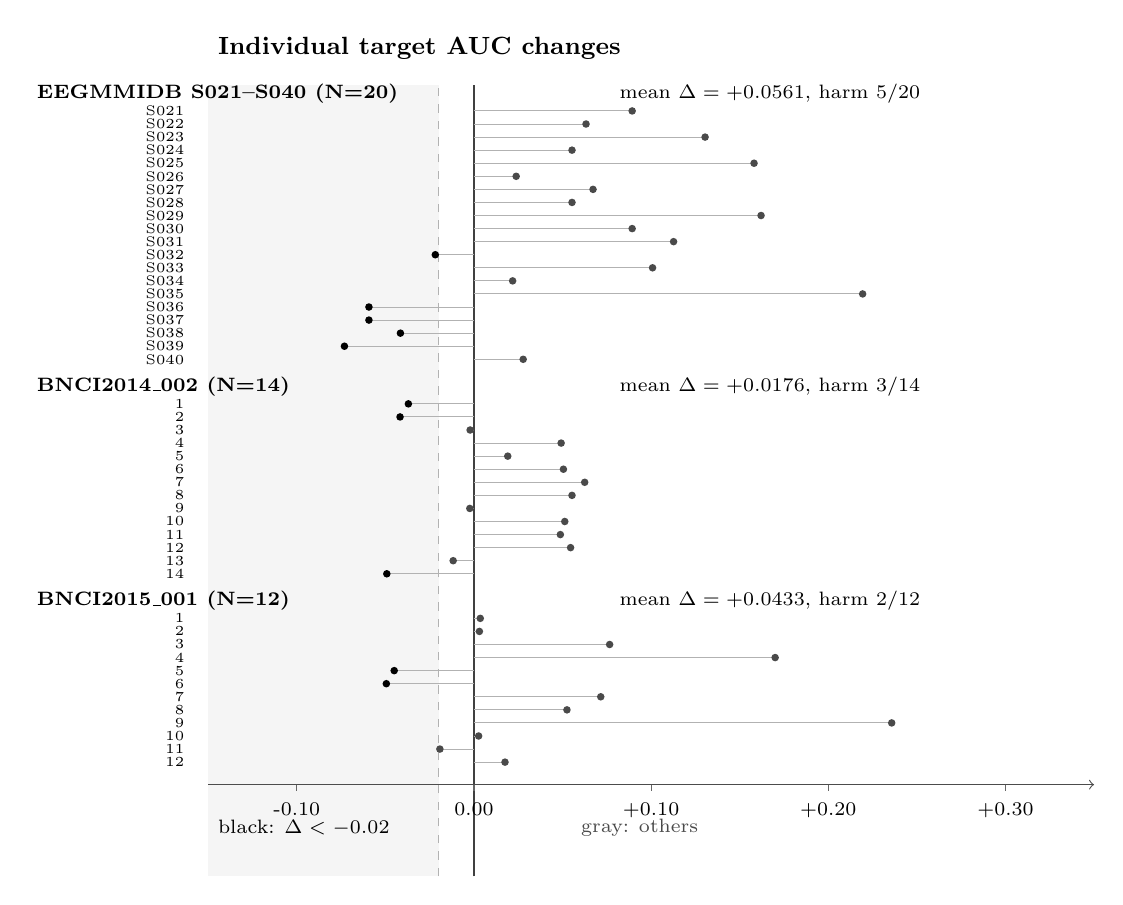
\begin{tikzpicture}[x=1cm,y=1cm]
\fill[gray!8] (2.300,1.68) rectangle (5.225,11.73);
\draw[dashed, gray!60] (5.225,1.68) -- (5.225,11.73);
\draw[black!75,line width=0.55pt] (5.675,1.68) -- (5.675,11.73);
\node[anchor=west,font=\small\bfseries] at (2.3,12.2) {Individual target AUC changes};
\node[anchor=west,font=\scriptsize\bfseries] at (0.0,11.620) {EEGMMIDB S021--S040 (N=20)};
\node[anchor=west,font=\scriptsize] at (7.4,11.620) {mean $\Delta=+0.0561$, harm 5/20};
\node[anchor=east,font=\tiny] at (2.12,11.400) {S021};
\draw[black!30,line width=0.35pt] (5.675,11.400) -- (7.684,11.400);
\fill[gray!58!black] (7.684,11.400) circle (0.048);
\node[anchor=east,font=\tiny] at (2.12,11.234) {S022};
\draw[black!30,line width=0.35pt] (5.675,11.234) -- (7.098,11.234);
\fill[gray!58!black] (7.098,11.234) circle (0.048);
\node[anchor=east,font=\tiny] at (2.12,11.068) {S023};
\draw[black!30,line width=0.35pt] (5.675,11.068) -- (8.610,11.068);
\fill[gray!58!black] (8.610,11.068) circle (0.048);
\node[anchor=east,font=\tiny] at (2.12,10.902) {S024};
\draw[black!30,line width=0.35pt] (5.675,10.902) -- (6.920,10.902);
\fill[gray!58!black] (6.920,10.902) circle (0.048);
\node[anchor=east,font=\tiny] at (2.12,10.736) {S025};
\draw[black!30,line width=0.35pt] (5.675,10.736) -- (9.232,10.736);
\fill[gray!58!black] (9.232,10.736) circle (0.048);
\node[anchor=east,font=\tiny] at (2.12,10.570) {S026};
\draw[black!30,line width=0.35pt] (5.675,10.570) -- (6.211,10.570);
\fill[gray!58!black] (6.211,10.570) circle (0.048);
\node[anchor=east,font=\tiny] at (2.12,10.404) {S027};
\draw[black!30,line width=0.35pt] (5.675,10.404) -- (7.187,10.404);
\fill[gray!58!black] (7.187,10.404) circle (0.048);
\node[anchor=east,font=\tiny] at (2.12,10.238) {S028};
\draw[black!30,line width=0.35pt] (5.675,10.238) -- (6.920,10.238);
\fill[gray!58!black] (6.920,10.238) circle (0.048);
\node[anchor=east,font=\tiny] at (2.12,10.072) {S029};
\draw[black!30,line width=0.35pt] (5.675,10.072) -- (9.321,10.072);
\fill[gray!58!black] (9.321,10.072) circle (0.048);
\node[anchor=east,font=\tiny] at (2.12,9.906) {S030};
\draw[black!30,line width=0.35pt] (5.675,9.906) -- (7.684,9.906);
\fill[gray!58!black] (7.684,9.906) circle (0.048);
\node[anchor=east,font=\tiny] at (2.12,9.740) {S031};
\draw[black!30,line width=0.35pt] (5.675,9.740) -- (8.210,9.740);
\fill[gray!58!black] (8.210,9.740) circle (0.048);
\node[anchor=east,font=\tiny] at (2.12,9.574) {S032};
\draw[black!30,line width=0.35pt] (5.675,9.574) -- (5.184,9.574);
\fill[black] (5.184,9.574) circle (0.048);
\node[anchor=east,font=\tiny] at (2.12,9.408) {S033};
\draw[black!30,line width=0.35pt] (5.675,9.408) -- (7.943,9.408);
\fill[gray!58!black] (7.943,9.408) circle (0.048);
\node[anchor=east,font=\tiny] at (2.12,9.242) {S034};
\draw[black!30,line width=0.35pt] (5.675,9.242) -- (6.166,9.242);
\fill[gray!58!black] (6.166,9.242) circle (0.048);
\node[anchor=east,font=\tiny] at (2.12,9.076) {S035};
\draw[black!30,line width=0.35pt] (5.675,9.076) -- (10.611,9.076);
\fill[gray!58!black] (10.611,9.076) circle (0.048);
\node[anchor=east,font=\tiny] at (2.12,8.910) {S036};
\draw[black!30,line width=0.35pt] (5.675,8.910) -- (4.341,8.910);
\fill[black] (4.341,8.910) circle (0.048);
\node[anchor=east,font=\tiny] at (2.12,8.744) {S037};
\draw[black!30,line width=0.35pt] (5.675,8.744) -- (4.341,8.744);
\fill[black] (4.341,8.744) circle (0.048);
\node[anchor=east,font=\tiny] at (2.12,8.578) {S038};
\draw[black!30,line width=0.35pt] (5.675,8.578) -- (4.741,8.578);
\fill[black] (4.741,8.578) circle (0.048);
\node[anchor=east,font=\tiny] at (2.12,8.412) {S039};
\draw[black!30,line width=0.35pt] (5.675,8.412) -- (4.030,8.412);
\fill[black] (4.030,8.412) circle (0.048);
\node[anchor=east,font=\tiny] at (2.12,8.246) {S040};
\draw[black!30,line width=0.35pt] (5.675,8.246) -- (6.300,8.246);
\fill[gray!58!black] (6.300,8.246) circle (0.048);
\node[anchor=west,font=\scriptsize\bfseries] at (0.0,7.900) {BNCI2014\_002 (N=14)};
\node[anchor=west,font=\scriptsize] at (7.4,7.900) {mean $\Delta=+0.0176$, harm 3/14};
\node[anchor=east,font=\tiny] at (2.12,7.680) {1};
\draw[black!30,line width=0.35pt] (5.675,7.680) -- (4.842,7.680);
\fill[black] (4.842,7.680) circle (0.048);
\node[anchor=east,font=\tiny] at (2.12,7.514) {2};
\draw[black!30,line width=0.35pt] (5.675,7.514) -- (4.736,7.514);
\fill[black] (4.736,7.514) circle (0.048);
\node[anchor=east,font=\tiny] at (2.12,7.348) {3};
\draw[black!30,line width=0.35pt] (5.675,7.348) -- (5.626,7.348);
\fill[gray!58!black] (5.626,7.348) circle (0.048);
\node[anchor=east,font=\tiny] at (2.12,7.182) {4};
\draw[black!30,line width=0.35pt] (5.675,7.182) -- (6.782,7.182);
\fill[gray!58!black] (6.782,7.182) circle (0.048);
\node[anchor=east,font=\tiny] at (2.12,7.016) {5};
\draw[black!30,line width=0.35pt] (5.675,7.016) -- (6.104,7.016);
\fill[gray!58!black] (6.104,7.016) circle (0.048);
\node[anchor=east,font=\tiny] at (2.12,6.850) {6};
\draw[black!30,line width=0.35pt] (5.675,6.850) -- (6.811,6.850);
\fill[gray!58!black] (6.811,6.850) circle (0.048);
\node[anchor=east,font=\tiny] at (2.12,6.684) {7};
\draw[black!30,line width=0.35pt] (5.675,6.684) -- (7.081,6.684);
\fill[gray!58!black] (7.081,6.684) circle (0.048);
\node[anchor=east,font=\tiny] at (2.12,6.518) {8};
\draw[black!30,line width=0.35pt] (5.675,6.518) -- (6.920,6.518);
\fill[gray!58!black] (6.920,6.518) circle (0.048);
\node[anchor=east,font=\tiny] at (2.12,6.352) {9};
\draw[black!30,line width=0.35pt] (5.675,6.352) -- (5.622,6.352);
\fill[gray!58!black] (5.622,6.352) circle (0.048);
\node[anchor=east,font=\tiny] at (2.12,6.186) {10};
\draw[black!30,line width=0.35pt] (5.675,6.186) -- (6.828,6.186);
\fill[gray!58!black] (6.828,6.186) circle (0.048);
\node[anchor=east,font=\tiny] at (2.12,6.020) {11};
\draw[black!30,line width=0.35pt] (5.675,6.020) -- (6.772,6.020);
\fill[gray!58!black] (6.772,6.020) circle (0.048);
\node[anchor=east,font=\tiny] at (2.12,5.854) {12};
\draw[black!30,line width=0.35pt] (5.675,5.854) -- (6.902,5.854);
\fill[gray!58!black] (6.902,5.854) circle (0.048);
\node[anchor=east,font=\tiny] at (2.12,5.688) {13};
\draw[black!30,line width=0.35pt] (5.675,5.688) -- (5.411,5.688);
\fill[gray!58!black] (5.411,5.688) circle (0.048);
\node[anchor=east,font=\tiny] at (2.12,5.522) {14};
\draw[black!30,line width=0.35pt] (5.675,5.522) -- (4.568,5.522);
\fill[black] (4.568,5.522) circle (0.048);
\node[anchor=west,font=\scriptsize\bfseries] at (0.0,5.176) {BNCI2015\_001 (N=12)};
\node[anchor=west,font=\scriptsize] at (7.4,5.176) {mean $\Delta=+0.0433$, harm 2/12};
\node[anchor=east,font=\tiny] at (2.12,4.956) {1};
\draw[black!30,line width=0.35pt] (5.675,4.956) -- (5.755,4.956);
\fill[gray!58!black] (5.755,4.956) circle (0.048);
\node[anchor=east,font=\tiny] at (2.12,4.790) {2};
\draw[black!30,line width=0.35pt] (5.675,4.790) -- (5.744,4.790);
\fill[gray!58!black] (5.744,4.790) circle (0.048);
\node[anchor=east,font=\tiny] at (2.12,4.624) {3};
\draw[black!30,line width=0.35pt] (5.675,4.624) -- (7.398,4.624);
\fill[gray!58!black] (7.398,4.624) circle (0.048);
\node[anchor=east,font=\tiny] at (2.12,4.458) {4};
\draw[black!30,line width=0.35pt] (5.675,4.458) -- (9.500,4.458);
\fill[gray!58!black] (9.500,4.458) circle (0.048);
\node[anchor=east,font=\tiny] at (2.12,4.292) {5};
\draw[black!30,line width=0.35pt] (5.675,4.292) -- (4.662,4.292);
\fill[black] (4.662,4.292) circle (0.048);
\node[anchor=east,font=\tiny] at (2.12,4.126) {6};
\draw[black!30,line width=0.35pt] (5.675,4.126) -- (4.562,4.126);
\fill[black] (4.562,4.126) circle (0.048);
\node[anchor=east,font=\tiny] at (2.12,3.960) {7};
\draw[black!30,line width=0.35pt] (5.675,3.960) -- (7.285,3.960);
\fill[gray!58!black] (7.285,3.960) circle (0.048);
\node[anchor=east,font=\tiny] at (2.12,3.794) {8};
\draw[black!30,line width=0.35pt] (5.675,3.794) -- (6.856,3.794);
\fill[gray!58!black] (6.856,3.794) circle (0.048);
\node[anchor=east,font=\tiny] at (2.12,3.628) {9};
\draw[black!30,line width=0.35pt] (5.675,3.628) -- (10.980,3.628);
\fill[gray!58!black] (10.980,3.628) circle (0.048);
\node[anchor=east,font=\tiny] at (2.12,3.462) {10};
\draw[black!30,line width=0.35pt] (5.675,3.462) -- (5.734,3.462);
\fill[gray!58!black] (5.734,3.462) circle (0.048);
\node[anchor=east,font=\tiny] at (2.12,3.296) {11};
\draw[black!30,line width=0.35pt] (5.675,3.296) -- (5.242,3.296);
\fill[gray!58!black] (5.242,3.296) circle (0.048);
\node[anchor=east,font=\tiny] at (2.12,3.130) {12};
\draw[black!30,line width=0.35pt] (5.675,3.130) -- (6.069,3.130);
\fill[gray!58!black] (6.069,3.130) circle (0.048);
\draw[->,black!70] (2.300,2.844) -- (13.550,2.844);
\draw[black!60] (3.425,2.844) -- (3.425,2.764);
\node[anchor=north,font=\scriptsize] at (3.425,2.734) {-0.10};
\draw[black!60] (5.675,2.844) -- (5.675,2.764);
\node[anchor=north,font=\scriptsize] at (5.675,2.734) {0.00};
\draw[black!60] (7.925,2.844) -- (7.925,2.764);
\node[anchor=north,font=\scriptsize] at (7.925,2.734) {+0.10};
\draw[black!60] (10.175,2.844) -- (10.175,2.764);
\node[anchor=north,font=\scriptsize] at (10.175,2.734) {+0.20};
\draw[black!60] (12.425,2.844) -- (12.425,2.764);
\node[anchor=north,font=\scriptsize] at (12.425,2.734) {+0.30};
\node[anchor=west,font=\scriptsize,black] at (2.300,2.294) {black: $\Delta<-0.02$};
\node[anchor=west,font=\scriptsize,gray!58!black] at (6.912,2.294) {gray: others};
\end{tikzpicture}
\caption{Paired participant-level target AUC differences between the frozen source participant-macro selector and the historical class-centred CovScore selector in three EEG cohorts. Five of 20, three of 14 and two of 12 participants, respectively, lost more than 0.02 AUC. The vertical reference line is zero, and the tinted region denotes the material-harm threshold. All three cohorts had been previously examined at project level; a within-run source lock does not turn the participant effects into externally preregistered confirmations. Historical Holm-adjusted results remain retrospective evidence. Points are descriptive and must not be treated as independent trials or a new confirmatory family.}
\label{fig:participant-harm-v10}
\end{figure*}


\subsection{Retrospective real-EEG check of the properly predictive comparator}
\label{sec:v18-fair-predictive}
The original class-centred comparator does not account for
between-source-person class-mean shifts
(Section~\ref{sec:v17-mean-shift-decomposition}, Eq.~\eqref{eq:v17-exact-nll-shift}).
We therefore executed a \emph{new secondary, post-outcome} comparison
of the correctly defined $C_{\mathrm{pred}}$ selector on public
Shin2017A EEG using the original, independent previously executed
preprocessing and classifier implementation. This additional
analysis is neither a new dataset nor a renewal of the earlier
confirmatory study. The Shin2017A outcomes had been seen before
the new score was specified.

For each of 29 outer held participants, the entire source-only
tangent reference and within-class state were reconstructed using
the other 28 participants. The source-participant-grouped inner
validation used only source-person trial labels; for each held
\emph{source} validation fold, the class means appearing in
Eq.~\eqref{eq:v16-conditional-prediction} were fitted exclusively
on the corresponding inner \emph{training} source groups.
The candidate set was that fold's originally source-feasible
27-point shrinkage grid, and the per-person proper-predictive
Gaussian log scores were averaged with equal source-person
weight. All 29 selected shrinkage strengths were serialised to
a machine-readable file and locked with SHA-256
\texttt{fac20e7f1ec1e43f3fa01af8ce88e44869e80f624d9a10b6123a57a6687f9b5c}
before re-opening the immutable original ZIP and reading the
outer target AUC outcomes. The original class-centred comparator
and source-macro policy were unchanged; the original Shin
score archive retained its previously verified SHA-256.



We also compared the two source-validation score
paths themselves, at the \emph{same} $\lambda=0.2$,
using the immutable original and new source-grouped
receipts. The genuine predictive Gaussian log score
exceeded the validation-class-centred covariance score
in 29/29 outer training pools. The mean difference
was $+0.86995$ per feature, ranging from $+0.83371$
to $+0.94214$. This is the nonnegative class-mean
shift penalty of Eq.~\eqref{eq:v17-exact-nll-shift}
measured on \emph{real EEG source validation data}.
These 29 source pools overlap heavily; neither their
positive signs nor the numerical penalty imply
a new independent dataset replication or a causal
guarantee of higher held-person AUC.

The newly implemented proper-predictive objective selected
\(\lambda=0.2\) in \emph{all 29} outer folds. It differs from the
original class-centred covariance choice in 29/29 folds, yet its
person-macro target AUC of \(0.786207\) was almost identical
to the source-macro policy's \(0.785900\). Proper predictive
scoring exceeded the original class-centred covariance
selection by \(0.022529\) person-macro AUC. In this
single previously exposed EEG dataset, the large comparison
against the class-centred score therefore does
\emph{not} translate into a discrimination-selector advantage
against genuine predictive likelihood.

The agreement between the two better-performing methods
should not be misrepresented as a general statistical
equivalence or proven non-inferiority. The new result
contains no new hypothesis test or adjusted $p$-value,
and equal source-population folds remain strongly dependent.
All 29 proper-predictive choices being 0.2 demonstrates
\emph{selection stability on highly overlapping training pools},
not successful participant-specific adaptation.
This new comparison narrows the paper's conclusion to
the \emph{measurement target itself}: a held-source
class-centred covariance log score can omit the
class-mean-shift penalty, changing the selected
regularisation regime and biasing the interpretation
of EEG decoding method comparisons.


\subsection{Second real EEG source-mean predictive comparison}
\label{sec:v18-bnci-proper}
We repeated the corrected source-mean Gaussian predictive
criterion on the \emph{original, separately frozen}
BNCI2014\_002 frontier experiment. Its public EEG pipeline
contained 14 held persons, 2240 trials and the original
source-only tangent-LDA scoring family. The new analysis
was specified \emph{after} this dataset's outcomes were
available; thus the original experiment's true-pre-data
status does not carry over to the new comparator.
The corresponding original artifact and new source-choice
files were independently read, with 14 paired AUC values
verified against the original immutable target AUC paths.

\begin{table}[tb]
\centering
\small
\caption{Matched real EEG descriptive comparisons after
correcting the covariance validation estimand. Entries
for the properly predictive criterion are \emph{post-outcome}
secondary analyses. The two rows correspond to different
public datasets, not two independent pre-data confirmations
of the new criterion. Mean source log-score penalty is
\(C_{\rm pred}-C_{\rm cent}\) at the newly chosen shrinkage
value, normalised per feature; positive values are an
exact class-mean-shift consequence.}
\label{tab:v18-two-real-cohorts}
\begin{tabular}{lcc}
\toprule
Metric & Shin2017A & BNCI2014\_002\\
\midrule
Held persons & 29 & 14\\
Source-macro selected AUC & 0.785900 & 0.778705\\
Proper predictive selected AUC & 0.786207 & 0.771886\\
Historical class-centred AUC & 0.763678 & 0.761116\\
Macro minus proper AUC & $-0.000307$ & $+0.006819$\\
Proper minus historical AUC & $+0.022529$ & $+0.010770$\\
Mean source class-mean-shift penalty & $+0.86995$ & $+0.91218$\\
Positive source penalties / folds & 29/29 & 14/14\\
\bottomrule
\end{tabular}
\end{table}

On BNCI2014\_002, the corrected proper-predictive
criterion selected \(\lambda=0.3\) in five folds,
\(0.4\) in eight, and \(0.5\) in one, contrasting
with the uniform \(0.2\) on Shin2017A.
Its person-macro AUC was \(0.771886\), compared
with \(0.778705\) under source-macro selection.
The difference of \(+0.006819\) AUC in favour
of source-macro selection is \emph{descriptive}.
An exploratory bootstrap over the 14 held persons,
conditional on their overlapping source fits,
gave the interval \([-0.00595,0.02027]\) AUC,
which includes zero. It cannot be interpreted
as a predeclared test, an equivalence result or
a population-level confidence interval.

At the same chosen \(\lambda\) within each
outer fold, the proper source log score
was higher than the class-centred score in
14/14 folds. The mean nonnegative difference
was \(+0.91218\) per feature, with foldwise
range \(+0.86056\) to \(+1.00008\).
This observation supports the algebraic
source-mean-shift decomposition in a second
public EEG dataset; it does \emph{not}
establish that the penalty predicts the
direction of target AUC gains.

The original BNCI2014\_002 frontier archive
used in this secondary comparison has its
own stored source-selection settings and
reported AUCs. It must not be silently
substituted for the separate originally frozen
two-BNCI testing-family statistics reported
above (for example, their originally
adjusted nonsignificant tests). Both
pre-existing score families are preserved
under their exact artifact identities,
and the corrected baseline is not added
retroactively to either family.


\subsection{Exact source-only estimand continuation and decision thresholds}
\label{sec:v19-estimand-homotopy}
The real-source identity in Eq.~\eqref{eq:v17-exact-nll-shift}
gives more than a post hoc contrast between two discrete
regularisation criteria. For each inner held-source participant
group $g$, let the historical covariance score be
$C_{0,g}(\lambda)$ and its nonnegative mean-shift penalty
be $P_g(\lambda)=C_{1,g}(\lambda)-C_{0,g}(\lambda)$.
On the original fixed source-feasible regularisation grid
$\Lambda_g$, define an \emph{estimand continuation}:
\begin{equation}
\label{eq:v19-estimand-continuation}
  J_{\alpha,g}(\lambda)=C_{0,g}(\lambda)
                +\alpha P_g(\lambda),\qquad
  \widehat\lambda_g(\alpha)
     \in\arg\min_{\lambda\in\Lambda_g}J_{\alpha,g}(\lambda),
  \quad \alpha\in[0,1].
\end{equation}
This is a \emph{diagnostic path of source-validation
measurements}, not a new participant-specific target
adaptation algorithm. At $\alpha=0$ it exactly recovers the
executed class-centred covariance selector; at $\alpha=1$
it exactly recovers source-trained-mean Gaussian predictive
selection. Neither choice requires an outer target example.

\paragraph{Finite-grid breakpoint theorem.}
Let $c_i=C_{0,g}(\lambda_i)$ and
$p_i=P_g(\lambda_i)$, both fixed by source data.
The optimized source score
$h_g(\alpha)=\min_i(c_i+\alpha p_i)$
is continuous, concave and piecewise affine.
Except at ties, the selected regularisation
$\widehat\lambda_g(\alpha)$ is piecewise constant.
All changes can occur only at candidate crossings
\[
\alpha_{ij}=\frac{c_j-c_i}{p_i-p_j}
\quad\text{where }p_i\ne p_j,\quad 0<\alpha_{ij}<1.
\]
Moreover the \emph{selected mean-shift penalty}
$p_{\widehat\lambda_g(\alpha)}$ cannot increase
as $\alpha$ grows. This defines a source-only,
exactly computable \emph{decision-stability
certificate}: $\alpha_g^*$ is the smallest
$\alpha$ at which the minimizer differs from
the original class-centred minimizer.

\emph{Proof.}
The pointwise minimum of finitely many affine
functions is a continuous concave piecewise-affine
function. Within each open interval between
pairwise crossings, candidate order is fixed.
For $a<b$, optimality at each endpoint gives
$c_i+a p_i\le c_j+a p_j$ and
$c_j+b p_j\le c_i+b p_i$, for minimizers
$i$ at $a$ and $j$ at $b$.
Adding both inequalities yields
$(b-a)(p_j-p_i)\le0$, so $p_j\le p_i$.
The other claims follow by enumerating the
finite pairwise line intersections.
\hfill$\square$

We computed the \emph{exact} lower envelope rather
than approximating its change points with an
arbitrary coarse $\alpha$ step. The original frozen
covariance score path and the separately executed
proper-predictive source-score path were paired at
the \emph{same} feasible scalar $\lambda$ in each
outer fold. An independent source-only program
enumerated all feasible affine crossings, merged
contiguous equal-minimizer intervals, and checked
the monotone-penalty theorem numerically on every
record. Each source-only trajectory was serialized
with a SHA-256 digest \emph{before} retrospective
joining of the already archived outer target AUC
paths. This chronology prevents within-execution
target-informed $\alpha$ decisions but does not
make the analysis prospectively pre-data.

\begin{table}[tb]
\centering
\small
\caption{Source-only exact estimand sensitivity in two
original EEG source pools. Thresholds $\alpha_g^*$ and
number of distinct minimizer intervals use only source
validation losses. The $\alpha$ grid is a diagnostic
continuation, not a calibrated target-optimal selector.
Outer folds overlap substantially and are not independent
laboratory replications.}
\label{tab:v19-homotopy-thresholds}
\begin{tabular}{lcc}
\toprule
Measure & Shin2017A & BNCI2014\_002\\
\midrule
Source-only outer folds & 29 & 14\\
Changes from $\alpha=0$ to 1 & 29/29 & 14/14\\
Median first-change $\alpha_g^*$ & 0.0660 & 0.1944\\
Minimum $\alpha_g^*$ & 0.0519 & 0.0406\\
Maximum $\alpha_g^*$ & 0.0930 & 0.2470\\
Source-regime intervals per fold & 6 & 7--9\\
\bottomrule
\end{tabular}
\end{table}

The real source-path measurements show a
strong dataset-dependent difference in the
sensitivity of the original covariance choice.
All 29 Shin2017A folds first changed their
selected $\lambda$ after an added penalty weight
between 0.0519 and 0.0930; the corresponding
range on BNCI2014\_002 was 0.0406--0.2470.
This does not mean the second dataset is
necessarily safer or more stable: the two
source populations and feature geometries
differ, and the threshold is a descriptive
decision property rather than a calibrated
measure of future-person predictive reliability.

For completeness, retrospective outcomes along
\emph{fixed, externally specified} diagnostic
weights $\alpha$ are shown in
Table~\ref{tab:v19-homotopy-outcomes}. These are
observations on already exposed held-subject
outcomes; no $\alpha$ was selected using target
AUC, no new adjusted $p$-value is calculated, and
no improvement relative to the executed proper
predictive comparator is claimed.
\begin{table}[tb]
\centering
\small
\caption{Person-macro target AUC along the source-only
estimand diagnostic path: retrospective outcomes,
\emph{not} a new trainable adaptive method result.
Endpoints reproduce the original class-centred
and the corrected proper-predictive comparators.}
\label{tab:v19-homotopy-outcomes}
\begin{tabular}{lcc}
\toprule
Fixed $\alpha$ & Shin2017A AUC & BNCI2014\_002 AUC\\
\midrule
0 (class-centred) & 0.763678 & 0.761116\\
0.1 & 0.772529 & 0.761518\\
0.4 & 0.777969 & 0.767333\\
0.8 & 0.784751 & 0.769933\\
1 (proper predictive) & 0.786207 & 0.771886\\
\bottomrule
\end{tabular}
\end{table}

The source path therefore yields an interpretable
\emph{measurement-stability diagnostic}: one can
report how small an explicit class-mean-shift
weight would change a published choice of
regularisation strength. It is not yet a
clinically deployable algorithm and adds no
prospectively validated EEG accuracy gain.


\subsection{A newly protocol-locked external acquisition cohort}
\label{sec:v20-new-external}
After establishing the exact source-estimand continuation
from the two previously exposed score archives, we locked
a new, independent public EEG experiment protocol in
GitHub \emph{before initiating the evaluation run} on
BNCI2014\_001 (BCI Competition IV Dataset 2a)
\cite{tangermann2012bciiv,jayaram2018moabb}.
This is a different acquisition dataset rather than a
resplit of Shin2017A or BNCI2014\_002. We restricted
the original four-class motor imagery paradigm to
left- versus right-hand imagery \emph{in the protocol},
before this run's results were computed, and used all
nine participants, 2,592 trials (288/person),
22 EEG channels and 8--30 Hz preprocessing.
The 22-channel covariance tangent vector contained
253 coordinates. The study used MOABB 1.7.2 and the
same original source-only covariance/tangent-space
LDA implementation, without target-fitted geometry.

For each held outer participant, the eight
remaining participants were divided into
five source-participant-grouped validation folds.
The source-only selected shrinkage values were:
(i) macro-AUC of the held \emph{source} people,
(ii) validation-class-centred Gaussian covariance
log score, and (iii) properly source-training-mean
Gaussian plug-in predictive log score.
All used the identical originally fixed finite
feasible shrinkage grid. In this run
we included analytic Ledoit--Wolf and OAS LDA
comparators, without additional optimization.
The nine source-only decisions were saved,
and the manifest was SHA-256 locked
(\texttt{d782c2e00c0cbdd7c3a7dc641e3ffc4e902ca8d075f61f65f78d8bb7d36216c0})
\emph{before the first outer target AUC was computed}.
The GitHub pre-run protocol SHA-256 was independently
reconciled with the release artifact.
No target label, target normalization, target
class mean or covariance informed model selection.

\begin{table}[tb]
\centering
\small
\caption{Newly run BNCI2014\_001 source-only
external EEG experiment (9 persons, 2,592 trials).
The experiment's protocol was committed before this
run's target evaluation; it was \emph{not}
independently preregistered or established
globally unexposed. Differences and harms are
descriptive: the same source people overlap
across outer folds.}
\label{tab:v20-new-cohort}
\begin{tabular}{lr}
\toprule
Selection or diagnostic & Result\\
\midrule
Source participant macro-AUC selector & 0.789052 AUC\\
Correct source-mean predictive score selector & 0.783415 AUC\\
Historical class-centred covariance selector & 0.772387 AUC\\
Analytic Ledoit--Wolf LDA & 0.752722 AUC\\
Analytic OAS LDA & 0.752829 AUC\\
Macro minus proper predictive (mean) & $+0.005637$ AUC\\
Conditional descriptive bootstrap interval & $[-0.00619,0.01793]$\\
Macro harmed more than 0.02 AUC vs proper & 1/9\\
Proper harmed more than 0.02 AUC vs macro & 2/9\\
Mean source log-score shift penalty & $+0.46946$\\
Median source first-change $\alpha_g^*$ & 0.14841\\
\bottomrule
\end{tabular}
\end{table}

Source discrimination selected
$\lambda=0.90$ for 3/9 folds,
0.95 for 5/9 and 0.98 for 1/9;
the correctly predictive source criterion
selected $\lambda=0.20$ for 3/9 folds
and 0.30 for 6/9, while the historical
class-centred criterion selected 0.10
for 7/9 folds and 0.15 for 2/9.
Thus the change in the \emph{measurement
estimand} again corresponded to a
different regularisation region.
The source mean-shift penalty was
positive in all nine groups as
\emph{required algebraically}; its
\emph{observed magnitude} was
0.46946 (per-feature log-score units)
when evaluated at the properly
predictive selected shrinkage.

The paired difference of
$+0.005637$ AUC between the
source-discrimination and correctly
predictive selectors had a post-run,
participant-conditional descriptive
bootstrap interval crossing zero.
We do \emph{not} report a newly
confirmatory superiority $p$-value or
claim equivalent predictive
performance. This first run
prespecified the preprocessing,
participants, target-information firewall,
method comparison and reporting
procedure, but it was not publicly
preregistered by an independent body;
we cannot certify that its outcomes
were never inspected elsewhere.
Its nine persons arise from one dataset
rather than independently sampled
clinical sites. The source-train-group
cross-validation fits overlap.

Together, the two retrospective
source-estimand correction studies
and this additional protocol-locked
new dataset support a narrower
conclusion than a new superior
EEG decoding method: the
historical class-centred criterion
systematically omits a mean-shift
component and can induce
different lambda choices in diverse
source populations. They do
not prove that any one of the
three selection objectives
always optimises future-person
discrimination or that its
empirical gain generalizes
to clinical deployment.


\subsection{A low-dimensional, risk-aware EEG stress test}
\label{sec:v21-lowrank-risk}
To challenge the possibility that the
estimand effect requires very high dimensionality,
we independently tested BNCI2014\_004,
BCI Competition IV Dataset 2b,
containing three bipolar EEG channels
and six covariance-tangent coordinates
\cite{tangermann2012bciiv,jayaram2018moabb}.
The 2026-10-12 repository-frozen first-run
protocol held each of nine people out,
using all available sessions. MOABB 1.7.2
returned 6,520 balanced trials (680--760
per person). These are measured per-person
counts, not the nominal catalogue total.

As a source-subject downside-risk
stress test, we added the following
fixed selector, alongside the original
macro-AUC, genuine source-mean Gaussian
predictive and historical validation
class-centred covariance scores:
\[
\widehat\lambda_{\mathrm{CVaR}}=
\arg\max_{\lambda\in\Lambda_{\rm src}}
\frac{A^{\rm src}_{(1)}(\lambda)+
A^{\rm src}_{(2)}(\lambda)}2 .
\]
Here $A^{\rm src}_{(j)}$ is the
$j$-th smallest held-source-person AUC
among eight SOURCE people in the fixed
five grouped folds. This is a
conventional worst-quarter CVaR
risk functional, \emph{not} an
independently novel learning operator.
Source-only choice vectors were SHA-256
locked before outer target AUC computation,
and the policy/grid were fixed before
this run. No target data entered model
or regularisation selection.

\begin{table}[tb]
\centering\small
\caption{New BNCI2014\_004 source-only
evaluation (9 people; 6,520 held-person
trials; 3 EEG channels, 6 tangent features).
All gains are descriptive, not independently
preregistered confirmation. CVaR stress
testing is a source-domain baseline.}
\label{tab:v21-lowdim-cvar}
\begin{tabular}{lr}
\toprule
Selection criterion & Mean AUC\\
\midrule
Held-source-person macro-AUC & 0.778002\\
Proper source-mean predictive Gaussian score & 0.776581\\
Worst-quarter source AUC (CVaR) & 0.777141\\
Historical source class-centred covariance & 0.770549\\
Ledoit--Wolf & 0.770628\\
OAS & 0.770640\\
\midrule
CVaR minus macro & $-0.000861$\\
CVaR minus macro, conditional bootstrap 95\% &
$[-0.00358,0.00067]$\\
CVaR selected a different $\lambda$ & 8/9 folds\\
$>0.02$ AUC harms relative to macro & 0/9\\
\bottomrule
\end{tabular}
\end{table}

The historical covariance criterion
selected $\lambda=0$ in all nine
source pools. The correctly predictive
Gaussian criterion selected 0.10--0.30
and source-macro discrimination
selected 0.50--0.80. The source CVaR
criterion changed the lambda choice
in 8/9 folds but \emph{did not
improve} mean held-person AUC,
nor the count of subject harms above
0.02 AUC. The class-mean-shift source
log-score penalty, evaluated at
properly selected shrinkage, was
nonnegative as required by algebra,
with empirical mean 0.92622 per feature.

These observations extend the
\emph{decision-instability mechanism}
to very low dimensional EEG geometry,
but reject a simplistic assumption
that source downside-risk optimization
must improve unseen-person AUC.
All nine source pools overlap and
there is one acquisition dataset,
not nine independent sites. The
protocol was committed before the
run, but was not independently
preregistered.

\subsection{An executed real-EEG rank-transition audit on held source participants}
\label{sec:v22-real-source-rank}
We executed the new pairwise source-rank audit on the original
BNCI2014\_002 covariance/tangent-LDA runner, preserving source-person
grouping, the same source-fitted representation, and the two
historical selection objectives. For each of 14 outer-held people,
the remaining 13 people constituted the \emph{source} pool. The
historical validation-class-centred covariance criterion and source
macro-AUC criterion were separately evaluated and selected from the
unchanged candidate grid on grouped inner source folds.
Pair-state transition matrices were then computed for the held
\emph{source} validation people only. The program verified that the
direct source-path AUCs match the reconstructed rank-based AUCs.

\begin{table}[tb]
\centering\small
\caption{V22 real BNCI2014\_002 source-validation diagnostics.
This table is a post-V21 explanatory SOURCE-domain calculation,
not a new unseen TARGET-person test. Gross churn is the
fraction of positive-negative pairs that change sign class;
macro AUC difference compares historical covariance-selected
to source-discrimination-selected regularisation.}
\label{tab:v22-source-rank}
\begin{tabular}{lrr}
\toprule
Audit unit & Source AUC difference & Gross churn\\
\midrule
First outer pool (13 held-source people) & $+0.04625$ & $15.35\%$\\
All 14 outer pools, mean & $+0.02680$ & $15.31\%$\\
\bottomrule
\end{tabular}
\end{table}

The full 14-pool job completed successfully, archived a source-only
JSON receipt with SHA-256
\texttt{15452a65fe43bb6f8e26f9f87deb65d73cec3a605966fa0060ee49805d72992f}
and passed identity, subject grouping and information-scope checks.
The reproducible execution record is GitHub Actions
\texttt{38273307665}. This is an exact attribution of
SOURCE-validation AUC differences to changed trial-pair ordering.
The 14 source pools are heavily overlapping, do not constitute
14 independent acquisition datasets, and do not establish any
new target AUC effect, target-harm prediction or statistical
significance. The results are useful as a mechanistic
implementation check, not as a claim of a successful new
regularisation method.

\subsection{Conditional continuous-search benchmark and a negative certification result}
\label{sec:v23-source-search-pilot}
The V23 source-only continuous-search pilot used exactly the
first outer pool of BNCI2014\_002, retaining 13 held
\emph{source} people, the original covariance/tangent-LDA
models, and a fixed $[0.05,0.95]$ feasible-search range.
After five interval splits with
$\epsilon=0.02$ source-macro-AUC target tolerance,
the original frozen 27-grid source-macro selector achieved
$0.79397$ AUC. The best lambda actually evaluated by
the continuous search achieved $0.79296$ source AUC.
The initial interval enclosure left a global source-macro
AUC upper bound of $0.88773$, or residual optimality
gap $0.09477$, so \emph{no certificate was issued}.

To address excessive conservatism, we subsequently
intersected the monotone spectral bounds with an
enclosing second-order Taylor interval; this is
\emph{post-pilot mathematical refinement}, not an
independent prospective validation. With the same
five-split budget, the source-macro upper bound fell
to $0.87939$, but the remaining optimality gap of
$0.08643$ still exceeded the declared tolerance.
The empirical selected-source AUC did \emph{not}
improve, and the method honestly remained inconclusive.
The refinement improves tightness on this example,
not target-person generalisation.

\begin{table}[tb]
\centering\small
\caption{Real BNCI2014\_002 held-source continuous search,
one outer training pool, five interval splits.
Source-validation only; not a new TARGET result.}
\label{tab:v23-source-search}
\begin{tabular}{lrr}
\toprule
Source-only operation & Empirical AUC & Upper residual gap\\
\midrule
Original 27-grid macro selector & 0.79397 & ---\\
Spectral interval, five splits & 0.79296 & 0.09477\\
Spectral $+$ Taylor, five splits & 0.79296 & 0.08643\\
\bottomrule
\end{tabular}
\end{table}

\subsection{Whole-cohort source-fold enclosure audit}
\label{sec:v23-full-taylor}
The original BNCI2014\_002 source-only continuum audit
was independently executed for all 14 outer-held-person
pools (13 SOURCE-validation people per outer pool) before
the post-pilot Taylor refinement. Using eight equal
lambda subintervals, the mean SOURCE positive--negative
pair fraction proven strictly sign-stable over the path
was $0.32166$; the held-source macro AUC change matched
V22 at $+0.02680$. Following the mathematical Taylor
refinement, a fully repeated 14-pool real EEG run
reproduced the identical AUC delta, with the stable
fraction increasing modestly to $0.32475$.

This $0.00309$ absolute increase in confirmed stability
is evidence of limited bound tightness improvement,
not an increase in decoding performance. The new
14-pool JSON receipt is SHA-256
\texttt{f8c54f027b359da036d09ff63ba43a50b65f565227b7d3b5aade6e936db04ae5}.
The trial-score bound is conditional on the source-fitted
models and held SOURCE people; it does not certify
future target-person accuracy or safety. In particular,
the majority of pairs remaining uncertified cannot be
called observed reversals.

\subsection{Independent-acquisition Weibo2014 source-locked test: no gain from finer optimisation}
\label{sec:v24-weibo}
The repository-fixed V24 first-run protocol specified Weibo2014
\cite{yi2014simplecompound,jayaram2018moabb} before any newly acquired
target outcomes were evaluated. It used all ten participants, the
fixed C3/Cz/C4 three-channel sensorimotor subset, left- versus
right-hand motor imagery, 8--30 Hz processing and a 160 Hz resample.
All 1,580 actually loaded trials were retained. This is a
different acquisition from the original cohorts, but deliberately
restricted to six covariance-tangent features and one binary task.
It is not an independent preregistered clinical trial.

All ten outer-held-person source-only parameter vectors were saved
and SHA-256 hashed before \emph{any} target scores were calculated.
The original 27-point held-source macro-AUC shrinkage choice,
a same-range, baseline-anchored continuous source optimiser,
source-trained-mean predictive Gaussian NLL, the historical
validation-class-centred covariance score, Ledoit--Wolf, OAS
and fixed $\lambda=0.50$ were evaluated on identical held-person
trials using the original tangent-LDA pipeline.

\begin{table}[tb]
\centering\small
\caption{V24 new Weibo2014 acquisition: mean held-person ROC-AUC,
$N=10$ people and 1,580 original MI trials. Models have identical
three-channel geometry and target information access (Z0).
These are descriptive first-run results, not independently
preregistered confirmation.}
\label{tab:v24-weibo}
\begin{tabular}{lr}
\toprule
Source-only selection policy & Held-person macro AUC\\
\midrule
Original 27-point source macro-AUC & 0.731405\\
V24 anchored continuous source AUC & 0.731405\\
Fixed $\lambda=0.50$ & 0.730149\\
Correct source-trained-mean Gaussian predictive NLL & 0.729358\\
Ledoit--Wolf & 0.725509\\
OAS & 0.725509\\
Historical validation-class-centred covariance & 0.725489\\
\midrule
V24 minus original grid & $0.000000$\\
V24 minus proper predictive NLL & $+0.002047$\\
\bottomrule
\end{tabular}
\end{table}

The conditional source-optimisation residual was at most
0.02 AUC on \emph{all ten} outer source pools, yet the
continuous optimiser selected the \emph{identical}
$\lambda$ as the 27-point source-macro baseline in
10/10 cases. The held-person AUC advantage over that
baseline was exactly zero in every person. Neither
method harmed a held individual by more than 0.02 AUC
relative to the other because their decisions were
identical. Against the correctly predictive Gaussian
selection, V24 had mean difference $+0.002047$; a
descriptive participant bootstrap interval was
$[-0.000234,0.004219]$, including zero. The corresponding
difference versus the historical class-centred score
was $+0.005916$; no individual difference in that
comparison exceeded 0.02 AUC in absolute magnitude.
The bootstrap intervals are conditional descriptive
statistics from ten overlapping-source LOSO fits;
they are \emph{not} a confirmatory population test.

This negative optimisation result is consequential:
more precise optimisation of a correctly defined
\emph{source} ranking criterion cannot be assumed
to yield a meaningfully better unknown-person
decoder. The result is consistent with the
distinction in Eq.~\eqref{eq:v24-transfer-gap},
but a small difference between policies alone
does not identify a causal mechanism of transfer.
We do not promote continuous optimisation to a
superior transfer algorithm.

An independent verifier downloaded the original
first-run Actions artifact, rechecked the ten
source-person selection records, recomputed all
held-person AUC macro means and the paired descriptive
statistics, and verified the pre-target selection
hash. The source-choice SHA-256 is
\texttt{a2fb5b334218a00b\ldots} (full digest in the online evidence ledger).
The original first-run Actions identifier is
\texttt{38279322314}; the independent verification
identifier is \texttt{38280133125}. The outcome
receipt was not used to revise the precommitted
selector or protocol. The acquisition/source
validity of its data is constrained by the
public dataset loader, not an independent
recollection of EEG.

\subsection{Real three-channel EEG source rank cells: a small numerical improvement}
\label{sec:v25-real-bernstein}
An executable retrospective source-only audit was completed on
Weibo2014 using the same original C3/Cz/C4 sensorimotor montage,
fixed six-dimensional tangent-LDA pipeline, and first outer
held-subject fold as the V24 first-run study. The other nine
participants each entered the original held-source validation
procedure, with source-fitted tangent references and shrinkage
spectra unchanged. Because Weibo2014 target outcomes had already
been exposed in V24, this audit is a \emph{post-outcome
mechanistic analysis}; it is not a new, independently untouched
external test or a prospective predictor of target harm.

\begin{table}[tb]
\centering\small
\caption{V25 3-channel Weibo2014 source-domain certificate
comparison, nine held-\emph{source} people, 12 fixed lambda
subintervals per range. Percentages count only pair rankings
conservatively proved invariant along an entire continuous
shrinkage interval. Failure to certify is \emph{not} an
observed rank crossing. There are no new target AUC effects
in this table.}
\label{tab:v25-source-bernstein}
\begin{tabular}{lrrr}
\toprule
Source interval & V23 Taylor & V25 Bernstein & Gain (pp)\\
\midrule
Complete $[0,1]$ & 94.121\% & 94.267\% & +0.146\\
Between source selectors & 96.274\% & 96.338\% & +0.064\\
\bottomrule
\end{tabular}
\end{table}

V25 gave a slightly higher certifiable pair fraction for
all nine validation source people on both prescribed
intervals, and reproduced the same endpoint AUC values
as V23 to the frozen numerical tolerance. These
increases are \emph{small}; no genuine future-person
generalisation effect, clinical value, computational
advantage or superior transfer selector has been
established. Neither method guarantees formal verified
floating-point arithmetic. The original completed
GitHub Actions proof-of-execution is
\texttt{38283087191}, with frozen JSON SHA-256
\texttt{c0c9e038376c899d}\ldots.
The full digest and source-person results remain in
the public immutable experiment artifact
\texttt{11762626131}.

The retrospective result motivates further mathematical
study of spectral rank boundaries, but does not justify
promoting the whole-numerator certificate into the
primary manuscript's EEG decoding performance claims.

\section{Recording identity, not person ID alone, is a prerequisite for EEG transfer validation}
\label{sec:v26-identity}
Contemporary EEG reproducibility work already documents that
trial-level validation can greatly overestimate subject-independent
performance \cite{gil2026subjectvalidation}; neither the
principle of leakage-safe splitting nor signal hashing is
presented here as novel. The previously unverified
\emph{record identity across different IDs} and its
consequences for this frozen regularisation comparison
are the dataset-specific methodological findings.

\paragraph{An independent raw-data integrity check.}
A separate source-locked Liu2024 acute-stroke experiment
originally included 50 public subject identifiers and
2,000 nominal trials (40 per identifier), with
29 EEG channels and no target-statistic fitting for
its \emph{predeclared} source regularisation rule.
The frozen 50-identifier outcome means were 0.59400
AUC for source-macro selection and 0.58985 for
genuine source-trained-mean Gaussian selection.
These are not yet estimates of transfer to 50
independent processed recordings.

We subsequently inspected each public MOABB 1.7.2
processed EEG trial array and the associated binary
left/right event labels \emph{without examining classifier
scores as a criterion for record grouping}. Exact
float64 array hashes, verified over all 50 identifiers,
found that IDs 4 and 5 have identical entire processed
EEG trial arrays and identical class labels.
No other full processed EEG array was repeated,
so the fixed release provides 49 unique preprocessed
recording groups under this exact identity criterion.
Although IDs 47 and 49 had coincident vectors of
reported target AUCs, their EEG signals differed
and they must remain distinct.
An independent released-EDF inspection found that
IDs 4 and 5 were in different binary EDF files but
32 of their 33 raw numerical channels were identical;
the sole differing channel was index 32 (zero-based),
with an empty name in the MNE EDF reader.
The comparison was performed on numerical signals,
not merely identical file names or matched classifier scores.
These tests do not identify human patients and do
not establish why the release contains identical
EEG waveforms under two subject IDs.

\paragraph{Why this can invalidate apparent held-person isolation.}
Let $D_i$ denote the preprocessed trial-signal and
label array associated with nominal subject ID $i$.
In the original leave-one-ID-out training protocol,
$\mathcal S_i=\{D_k:k\ne i\}$. For $D_i=D_j$ with
$i\ne j$, $D_j\in\mathcal S_i$ is a copy of the
nominal held-out record, including its labels.
The source-fitted tangent reference, spectral covariance,
class contrast, Gaussian predictive source criterion and
discriminative source validation can therefore all
depend on the held record through its duplicate.
The assumption of independent source/target
\emph{recordings} is violated even though the numerical
subject identifiers differ. For all other outer folds,
the same recording receives additional weight through
its duplicate IDs. Correcting only the denominator
of a reported mean AUC does not repair the fitted
source models.

\paragraph{Purged re-fitting.}
The precommitted retrospective V26 protocol groups
only exact signal- and label-identical records;
it retains the smallest ID per group, excludes
other identical copies \emph{from every source pool
and every target denominator}, and re-fits all
source references and source-only selection rules.
Every model uses one of the other 48 unique
processed recording groups as its held target
and is trained on the remaining 48.
All grouped source decisions are locked before
their corresponding target AUCs are joined.
Numerical results are not reported until the
real-data run and identity receipts have passed.

\paragraph{Information-budget limitation.}
Identifying duplicates required a global inspection
of the publicly released held-target EEG arrays;
therefore the new reanalysis is \emph{not} a strict
no-target-feature-access Z0 or an independent
prospective test. This retrospective integrity check
cannot prove causal performance inflation solely
from the duplicate: purging also changes source
sample weights and fitted covariance/geometry.
The previously exposed 50-identifier result
must be treated as \emph{unqualified} with respect
to recording-independent transfer until a
record-level separation analysis is complete.

\section{Checking partial EEG epoch replay beyond complete recording identity}
\label{sec:v27-epoch-identity}
The V26 check identified one pair of identical full
preprocessed EEG recording arrays under different subject identifiers.
That check is insufficient to exclude \emph{partial} record overlap:
two different 40-trial arrays can share a small number of identical
epochs while having different complete-record SHA-256 digests.
We distinguish EEG \emph{subject identifiers}, numerical
\emph{recording content}, and human patient identity; the last
cannot be determined from the published arrays.

\paragraph{Content-based epoch-overlap graph.}
For subject identifier $i$, let
$E_i=\{h(x_{it}):t=1,\ldots,n_i\}$ be the set of
cryptographic fingerprints of the complete EEG trial arrays
after the single, frozen MOABB preprocessing pipeline. The
fingerprint hashes both channel/time dimensions and the contiguous
float64 signal bytes. Candidate equality is checked by exact
numerical array comparison, with contradictory class labels
treated as a dataset-integrity failure.
Define the undirected graph with an edge $(i,j)$ if
$E_i\cap E_j\ne\varnothing$ for $i\ne j$.
The graph ignores observed classifier predictions and AUC values.

For any partition that assigns each complete identifier's
trials to one fold, \emph{zero exact trial-content overlap between
training and test folds} is equivalent to requiring that
every connected component of this graph is contained in
one fold. If an edge crosses the partition, its identical
epoch appears on both sides; conversely, if an exact epoch
appears on both sides, that pair defines a crossing edge.
A component can be separated only by cutting such an edge.
This elementary graph observation is not a newly invented
generalisation theorem. It gives an actionable grouping
contract under exact equality, which the original
complete-record check does not provide.

\paragraph{Audit and boundary.}
We precommitted a retrospective scan over all 50 public
Liu2024 subject IDs and all 2,000 originally retained
40-trial observations, before executing the new trial-level
scan. A pinned MOABB 1.7.2 loader retains the previous
29-channel, 8--30 Hz, 160 Hz left/right motor-imagery
processing and 20/20 class balance. For each exact epoch
content appearing under multiple identifiers, we count
shared unique epoch contents, cross-identifier matching
trial instances and any transitive groups. Internal repeats
are reported separately. No threshold is tuned to target
classifier performance, and no unverified near-duplicate
criterion is introduced. Synthetic tests inject
partial overlap, transitive reuse, whole-record copies,
and conflicting event labels. The entire source EEG
trial list and matching rules are fixed prior to the
audit, with complete reproducible logs archived.

All grouping necessarily inspects globally released
EEG signal content, including held records. Consequently,
any resulting component-aware reanalysis is an
\emph{exposed-cohort integrity sensitivity study},
not a physically target-isolated, independently
prospective zero-calibration experiment.
Exact equality says nothing about near duplicates,
overlapping-but-nonidentical time windows, patient
identity or source-site dependencies. Even a negative
additional-overlap scan would only strengthen one
specific data-integrity check and cannot be promoted
to a new AUC gain or proof of population transfer.

Published EEG validation research documents
the importance of the subject/record split
\cite{gil2026subjectvalidation}. Our novelty claim
is restricted to the \emph{specific} released-record
finding and its reproducible trial-granularity
consequences under a frozen EEG decoding pipeline,
not to the general concept of preventing leakage.

\subsection{Independent source-group attestation from exact EEG epoch identity}
\label{sec:v28-independent-graph}
We reconstructed the eligible held-record source splits from the
original V27 exact-epoch overlap ledger, without loading EEG waveforms,
using class labels for fitting, or consulting classifier AUCs.
The independent graph implementation creates an edge whenever two
identifiers have at least one exactly equal full processed EEG epoch.
Every connected component must remain within one validation fold
to prevent exact cross-boundary trial-content leakage.

The immutable public Liu2024 scan contains 50 nominal identifiers,
2,000 original trials and 1,960 distinct trial arrays. It reports
a single cross-identifier component $\{4,5\}$ sharing all 40 trials.
No other exactly equal partial trial-content reuse was detected.
Reconstruction therefore yields 49 held-record groups with 48
distinct source representatives per fold. All 49 split contracts
were checked successfully against the original V27 artifact in
GitHub Actions run \texttt{38288719062}. The independent
report SHA-256 begins with \texttt{5b50866f464a4d8f};
the complete digest and JSON reside in the public run artifact.

Synthetic tests deliberately insert partial and transitive
cross-record replay, duplicate graph edges and inconsistent
label counts. When two different complete records share just
one original epoch, the algorithm combines their components
instead of retaining an invalid subject-ID split.

This independent audit establishes a necessary split condition,
not the numerical performance of a refitted EEG decoder.
The separately committed V26 runner discarded all
copied records from source fitting and target reporting,
re-fitted the geometry and selection rules and SHA-locked
every source choice before joining target AUCs. The
additional V28 independent artifact cross-check
confirmed that all 49 actual source-training sets
match the graph-derived legal folds; see
Section~\ref{sec:v28-three-estimands}. These
checks remain retrospective and do not establish
any causal inflation estimate or new blinded test.

Global inspection of held EEG signal content was used in
this integrity analysis. It is retrospective and cannot
be represented as strict target-signal-isolated Z0.
Exact equality also does not identify human patients
or rule out approximate duplicates and overlapping
non-identical time windows.

\subsection{Complete real EEG re-fitting after exact-record deduplication}
\label{sec:v28-purged-actual}
The originally exposed Liu2024 50-identifier zero-target-label
comparison was subsequently found to contain identical complete
processed source/target recordings under IDs 4 and 5.
We have now completed an independent-run, retrospective
49-representative \emph{full model refit} under fixed
MOABB 1.7.2 preprocessing. For each held recording group,
48 other distinct representatives (1,920 source trials)
are used to re-fit the tangent reference, covariance
estimator, discriminant, predictive-source Gaussian score
and source-macro selection objective. The 49 selected source
policies were SHA-locked before 49 target AUC evaluations
were joined. No newly selected threshold or new test
cohort is introduced by this reanalysis.

\begin{table}[tb]
\centering\small
\caption{Original exposed 50-identifier average AUC and fully
retrained 49 unique-\emph{content} group retrospective average
AUC. The difference is a \emph{joint dataset-repair change},
not a causal estimate of leakage inflation; both original
target exposures and global record inspection were known.}
\label{tab:v28-fullrefit}
\begin{tabular}{lrr}
\toprule
Source-only criterion & Old 50 ID & Full 49-group refit\\
\midrule
Source-macro discrimination & 0.59400 & 0.58255\\
Proper source-mean predictive likelihood & 0.58985 & 0.58133\\
Historical class-centred covariance & 0.59305 & 0.58117\\
Ledoit--Wolf & 0.59085 & 0.57852\\
OAS & 0.58985 & 0.57827\\
\bottomrule
\end{tabular}
\end{table}

The original raw-source-fold study is GitHub Actions
\texttt{38285928569}, which completed successfully
and produced a frozen full-refit outcome manifest,
SHA-256 prefix \texttt{5cfdc41ca056fa39}
(full hash in the online evidence receipt).
The correct predictive comparator remains close to
source-macro selection; their 49-record descriptive
difference is $+0.00122449$ AUC.
This gives no evidence of a material, uniformly
beneficial new regularisation rule.

The original 50-ID outcome mean and new 49-group
mean change through two logically distinct operations:
(i) reweighting the reporting denominator by deleting
the copied target identifier while retaining the old
fitted models, and (ii) rebuilding the 49 training
source pools and refitting their geometry and policies.
The first is \emph{not} a leakage repair and the
second changes multiple aspects of the learned estimator.
A separate, fully hash-verified three-estimand comparison
will report each arithmetic contrast; until its
independent execution passes, this table must not
be interpreted as a decomposition or causal effect.

\subsection{Three-way decomposition of nominal and record-purged EEG outcomes}
\label{sec:v28-three-estimands}
After successful completion of the 49-record full refit, an
independent job downloaded \emph{three immutable experiment
artifacts}: the original 50-ID source-locked result, the
all-2,000-epoch identity ledger, and the 49-representative
fully refitted result. It reconstructed all 49 legitimate
train/held source partitions from exact EEG trial identity
and checked their equality to the actual source sets used
for the real-data re-fitting. All 49 passed, with source
policies SHA-locked before the recorded target AUCs.

For each frozen method, define three descriptive means.
$A$ is the original 50-identifier LOPO mean. $B$ drops
the copied target ID 5 from the old outcome table while
keeping all \emph{old fitted models} unchanged. $C$
recomputes tangent-space references, class-contrast
models and the source-only parameter choices from the
48 distinct source representatives for each of the 49
held recording groups. The arithmetic identity
\[
 C-A=(B-A)+(C-B)
\]
separates the reporting-denominator change from
the aggregate fully-refitted-model change on a
fixed set of 49 target IDs. It is \emph{not} a
causal decomposition of leakage inflation, since
the fit and source-selection changes themselves
combine several factors.

\begin{table}[tb]
\centering\small
\caption{Liu2024 exact-record identity sensitivity:
participant/record-content-macro AUC under original nominal
50-ID evaluation ($A$), old fitted models restricted
to 49 unique target rows ($B$), and complete 49-group
source refitting ($C$). All differences are retrospective
descriptive observations, not preregistered treatment effects.}
\label{tab:v28-three-estimands}
\begin{tabular}{lrrr}
\toprule
Criterion & A: 50 IDs & B: 49 target rows & C: 49 refit\\
\midrule
Source macro-AUC & 0.59400 & 0.58867 & 0.58255\\
True predictive Gaussian & 0.58985 & 0.58505 & 0.58133\\
Historical class-centred & 0.59305 & 0.58724 & 0.58117\\
Ledoit--Wolf & 0.59085 & 0.58495 & 0.57852\\
OAS & 0.58985 & 0.58378 & 0.57827\\
\bottomrule
\end{tabular}
\end{table}

For source-macro shrinkage, $B-A=-0.00532653$
and $C-B=-0.00612245$, summing to
$C-A=-0.01144898$ AUC. Crucially, re-fitting
altered the source-macro-selected shrinkage
in \emph{37 of 49} matched held recording groups.
The source-mean predictive Gaussian criterion's
selected shrinkage stayed identical in all
49 comparisons, although its mean AUC still
changed from $0.58985$ to $0.58133$.
Thus changes in selected $\lambda$ and
changes in fitted model geometry or target
performance are distinct events, in line
with the original objective-mismatch hypothesis.

An independent job \texttt{38289471605}
validated the old, held-content and refitted
source SHA manifests and the identity graph;
its frozen joint-audit report SHA-256 begins
\texttt{c9b49cf112e1e7d4} (full digest
in the online Actions artifact).
Neither these paired observations nor the
arithmetic identity can attribute performance
loss causally to a specific duplicated observation,
prove distinct patient identity, or guarantee
record-independent generalisation at another site.
This experiment was performed after the
target outcomes had been exposed and global
target signal identities inspected, not as
a new strict Z0 confirmatory trial.


\subsection{The key prospective spectral-representation prediction fails}
On the separate untouched S041--S060 block, four prespecified
configurations compared WIDE231, FB8-1848, source-PCA-matched
FB8-231 and nuisance-augmented WIDE-1848. The primary
difference-in-differences for FB8-vs-WIDE under discrimination versus
Ledoit--Wolf regularisation was \(-0.07781\) AUC
(95\% [-0.12415,-0.03451], Holm \(p=0.01328\)).
The selection objective materially affected the representation
conclusion, but in the \emph{opposite} direction to the historical
claim that discrimination-oriented regularisation would reveal a
universal filter-bank advantage. Dimensionality-matched and nuisance
controls also contradicted a monotonic feature-dimension explanation.

\subsection{External path variation lacks a confirmed population lower bound}
Observed BNCI2014\_002 and BNCI2015\_001 AUC-path ranges were
0.03844 and 0.05011, with empirical \(\delta_{0.02}\) equal
to 0.91611 and 0.17519 per-dimension source NLL-regret units.
Post-outcome path-wide bootstrap oscillation radii were 0.04035
and 0.05923. In both cohorts, the resulting conservative
lower range bound is zero; a population-wide effect over 0.02
cannot be claimed from these data.

\begin{table*}[t]
\centering
\caption{Original v5 405-candidate target AUC path spreads and V11 translation-invariant simultaneous-path sensitivity. Observed ranges are exact reconstructions from the raw TRUE PRE-DATA external experiment outputs; ordinary 20,000-resample percentile intervals for an empirical max--min statistic are shown only for provenance, not as simultaneous population confidence intervals. \(q_{\mathrm{osc}}\) is the nominal 95th percentile of the paired-bootstrap error-path oscillation; \(L_{\mathrm{osc}}=\max(0,\text{observed span}-q_{\mathrm{osc}})\) conditions on the fixed studied cohorts and is post-outcome.}
\label{tab:validity-frontier}
\small
\begin{tabular}{lrrrrr}
\hline
Cohort & \(N\) & Observed span & Prior percentile interval & \(q_{\mathrm{osc}}\) & \(L_{\mathrm{osc}}\) \\
\hline
BNCI2014\_002 & 14 & 0.0384 & [0.0271, 0.0666] & 0.0403 & 0.0000 \\
BNCI2015\_001 & 12 & 0.0501 & [0.0224, 0.1034] & 0.0592 & 0.0000 \\
\hline
\end{tabular}

\vspace{1mm}
\footnotesize
Original observed \(\delta_{0.02}\) fidelity-regret budgets are 0.9161 and 0.1752 raw per-dimension source NLL units; neither path crosses the 0.02 AUC threshold after the V11 oscillation correction. A zero conservative lower bound is inconclusive, not proof of a flat population path. The bootstrap does not account for overlapping source-model refits or across-dataset sampling uncertainty. All quantities are descriptive and no new confirmatory hypothesis test is introduced.
\end{table*}






\section{Discussion}
The central finding is not that discrimination-optimised covariance
shrinkage is universally preferable, but that \emph{an apparently
reasonable validation criterion can silently change the scientific
estimand}. The previously called Cov-NLL scored each held-source
participant after subtracting that participant's own validation-class
means. It therefore omitted an exact, nonnegative source-trained-mean
shift penalty and must not be compared to discriminative selection
as if it were proper predictive likelihood. The corrected source-trained
Gaussian score changes the magnitude and interpretation of the earlier
advantage. Selecting shrinkage using held-source discrimination is
classical; our contribution concerns the reproducibility and
interpretation of that objective comparison, not priority for
discriminative tuning \cite{friedman1989,tomioka2010regularized}.

The prospectively fixed EEGMMIDB comparison is real, but it also
contains harmed participants; the two original independently frozen
BNCI families do not individually establish adjusted superiority.
Shin2017A's proper predictive comparison is retrospective.
The subsequent three-channel CVaR experiment demonstrated
that changing the source-selected regularisation does not
necessarily change target discrimination, and the prospective
spectral-representation intervention refuted the initially
expected universal filter-bank advantage. These negative
results are central to the paper, not unsuccessful parameter
searches to be discarded.

The V22 and V23 mechanisms distinguish source parameter changes,
score-pair order changes and source-validation AUC effects.
The V24 continuous branch-and-bound repair provides a useful
conditional finite-\emph{source} optimisation gap. Yet the new
Weibo2014 experiment is more informative for its \emph{failure
to improve transfer}: the same shrinkage was selected
in every outer source pool by the new continuous method
and the original 27-point grid, producing identical
held-person predictions by that pipeline. The average
$+0.00205$ AUC contrast to proper predictive likelihood
has a descriptive participant interval containing zero.
Under the deterministic decomposition of
Eq.~\eqref{eq:v24-transfer-gap}, closing the source
optimisation term cannot bound the unobserved
source--target discrepancy; no source-only rank
certificate is an unseen-person safety guarantee.

The independent Weibo acquisition extends the practical
stress test to another recording site, but the fixed
three-channel, single binary MI task is deliberately
limited. Its ten overlapping-source leave-one-person-out
models do not provide ten independent study replications,
and repository protocol-first chronology is weaker than
independent preregistration. The work does not establish
SOTA deep EEG performance, calibration time saved,
clinical safety, or deployment-ready trigger policies.
The most robust methodological recommendation is to
specify validation estimands, target-information budgets,
pre-outcome selection boundaries, negative controls,
and participant-level adverse effects before making
claims about EEG regularisation.

\section{Conclusion}
An historical validation-class-centred EEG covariance score
was not a proper predictive Gaussian likelihood, and
the distinction changes how earlier discrimination-based
regularisation gains should be interpreted. Exact
pairwise ranking and spectral path analyses clarify why
source selection decisions can differ without producing
important target AUC improvements. The independently
audited ten-person Weibo2014 protocol-first test
found that source-optimality gaps were numerically
small but continuous selection and the original
27-point source grid chose identical parameters and
achieved the same held-person macro AUC.
This supports \emph{measurement correctness and
selection validity} as the manuscript's contribution,
not superiority of a new EEG decoder. Broader
multi-acquisition, fully independent pre-data
replication is required before claiming a universally
safe or better shrinkage rule.

\section*{Statements and Declarations}
\textbf{Data availability:} The EEG cohorts are publicly distributed.
Original participant score receipts, repository commit hashes and code
availability must be confirmed in the final submission package.

\textbf{Author contribution, funding, competing interests, ethics and
AI-assisted writing:} To be completed and confirmed by all authors before
publisher upload. No declaration is made on an author's behalf.

\bibliographystyle{unsrt}
\bibliography{references_v10}
\end{document}
